% \documentclass[12pt, oneside]{book}

\chapter{Equation of State}
\label{chap:EquationofState}

In this chapter we go back now and consider some fundamentals about water that are important to this course.  Seawater is a relatively complex substance.  As discussed before, lateral density differences can drive lateral circulation, hence it is important to understand and predict how those differences arise.  Further, the ocean is a huge reservoir of heat, and understanding its heat content is important for predicting weather and future climate.

\section{Temperature}

Temperature is a thermodynamic property of a substance, the value of which is proportional to the kinetic energy of the random motions of the molecules in the substance (these are called \Wikiref{Brownian motion}). The heat necessary to bring a substance to a given temperature is proportional to the \emph{\Wikiref{heat capacity}}.  In order to change a parcel of water's temperature by $\Delta T$, we need to supply energy proportional to the heat capacity of the water:
\begin{equation}
   \Delta E = c_p\ \Delta T
\end{equation}
where $c_p$ has units of $J\, C^{-1}\ kg^{-1}$, and $\Delta E$ has units of $J\ kg^{-1}$.  Values for $c_p$ are given in \fref{fig:HeatCapacity}, and note that the heat capacity is not constant, but depends on the temperature of the water, its salinity, and its pressure!  The dependence is non-linear, so we usually resort to using a computer to calculate the empirically-derived values.  However, for a litre of fresh water ($\approx 1\ kg$) at $20^oC$ we would need 4180 J of energy to raise the temperature by one degree.  

\begin{figure}
    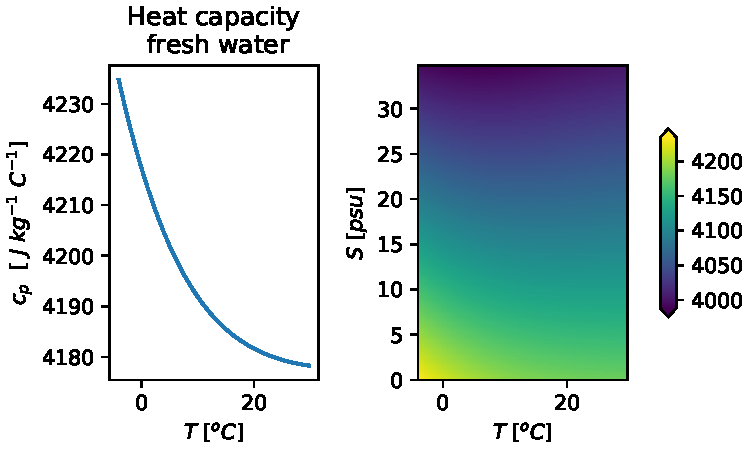
\includegraphics[width=3in]{./figs/HeatCapacity.pdf}
    \caption{Heat capacity of water a) for fresh water as a function of temperature, b) as a function of both salinity and temperature.  Both are presented at the sea surface.}
    \label{fig:HeatCapacity}
\end{figure}

The heat capacity of water is impressive compared to air, where typical values are $1000\ J\, C^{-1}\ kg^{-1}$.  The whole atmosphere has a weight of $\approx 10^{4} \ kg\ m^{-2}$, so heating the whole atmosphere one degree requires $\approx 10^7 J\ m^{-2}$.  Conversely, the ocean at 4000 m deep and with a density close to $1000 \ kg\,m^{-3}$ weighs approximately $4\times10^6\ kg\ m^{-2}$, so raising its temperature by one degree requires $16\times10^9 J\ m^{-2}$, more than three orders of magnitude more energy.  This helps explain why the ocean is such an important reservoir of heat in the climate system.  

\subsection{Measurement}

\begin{figure}[hbtp]
  \begin{center}
    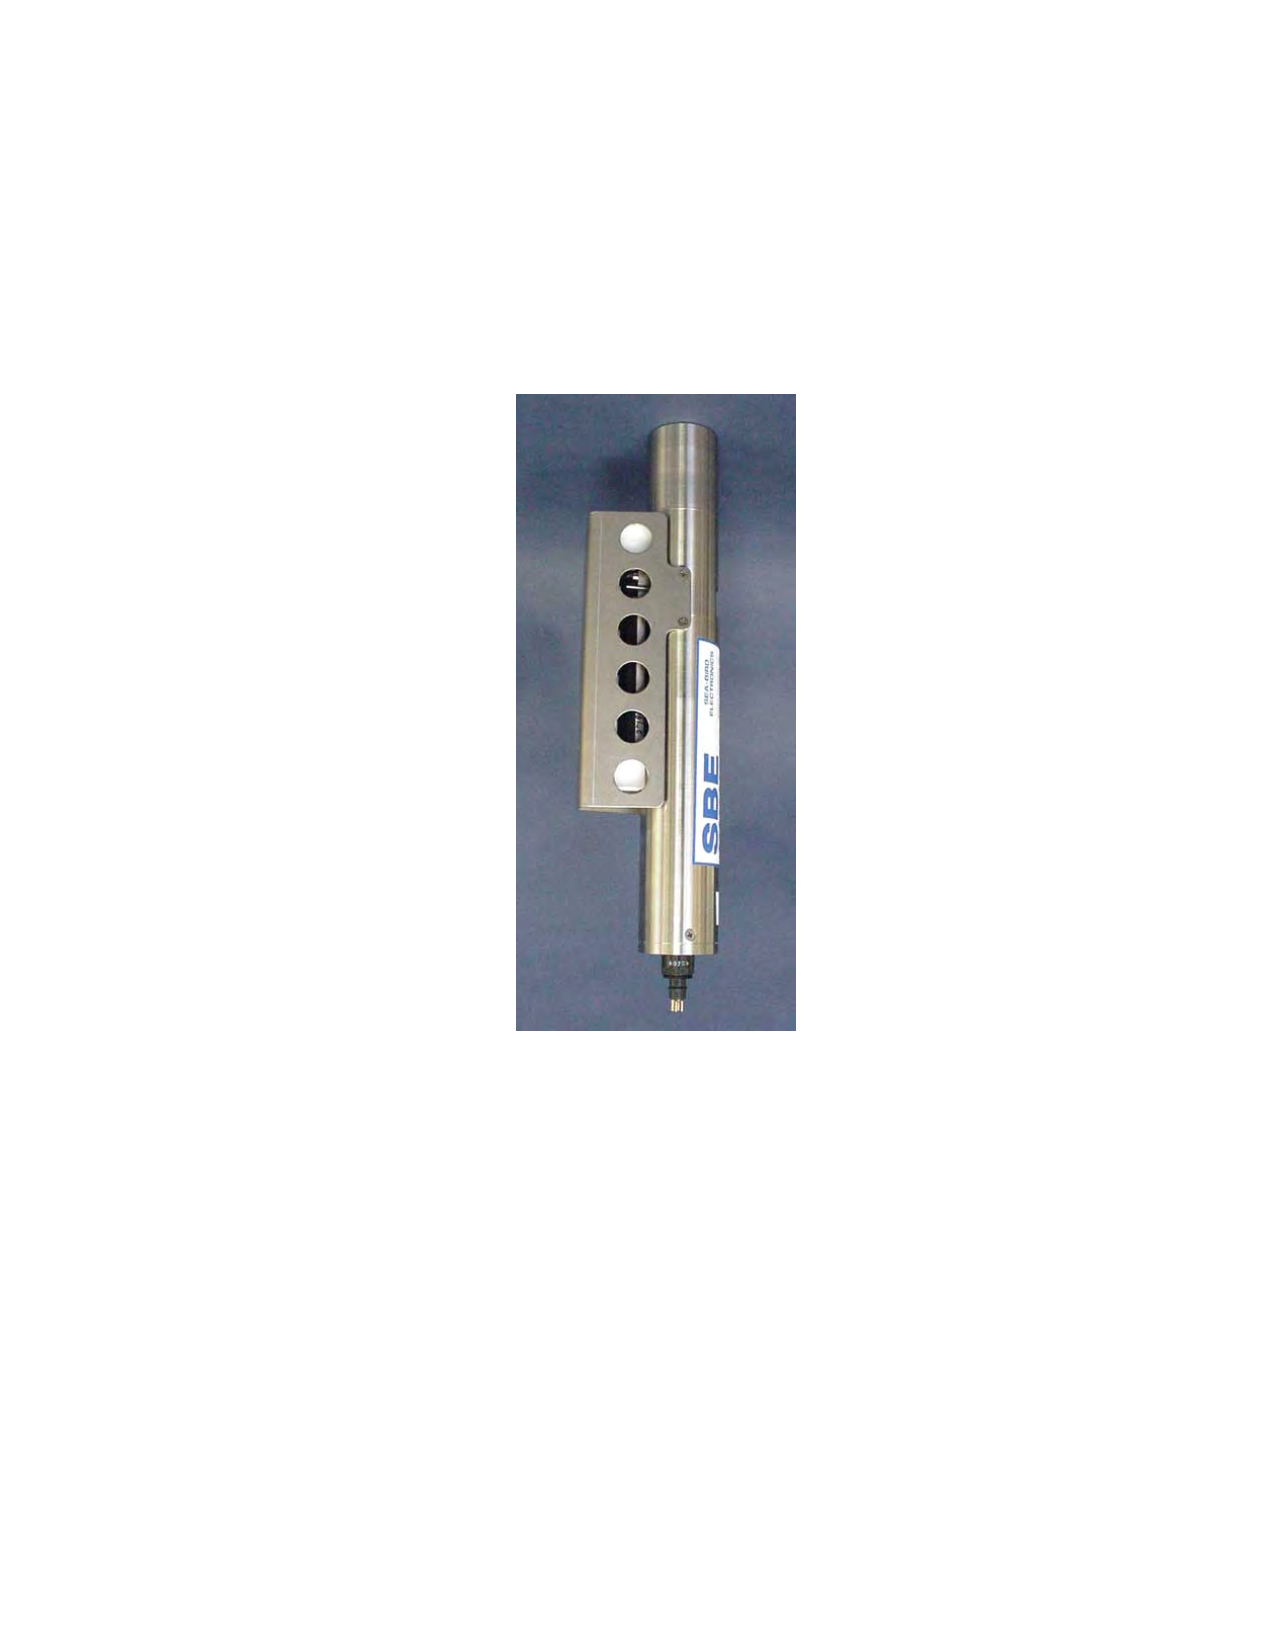
\includegraphics[width=1in]{figs/CTD.pdf}
    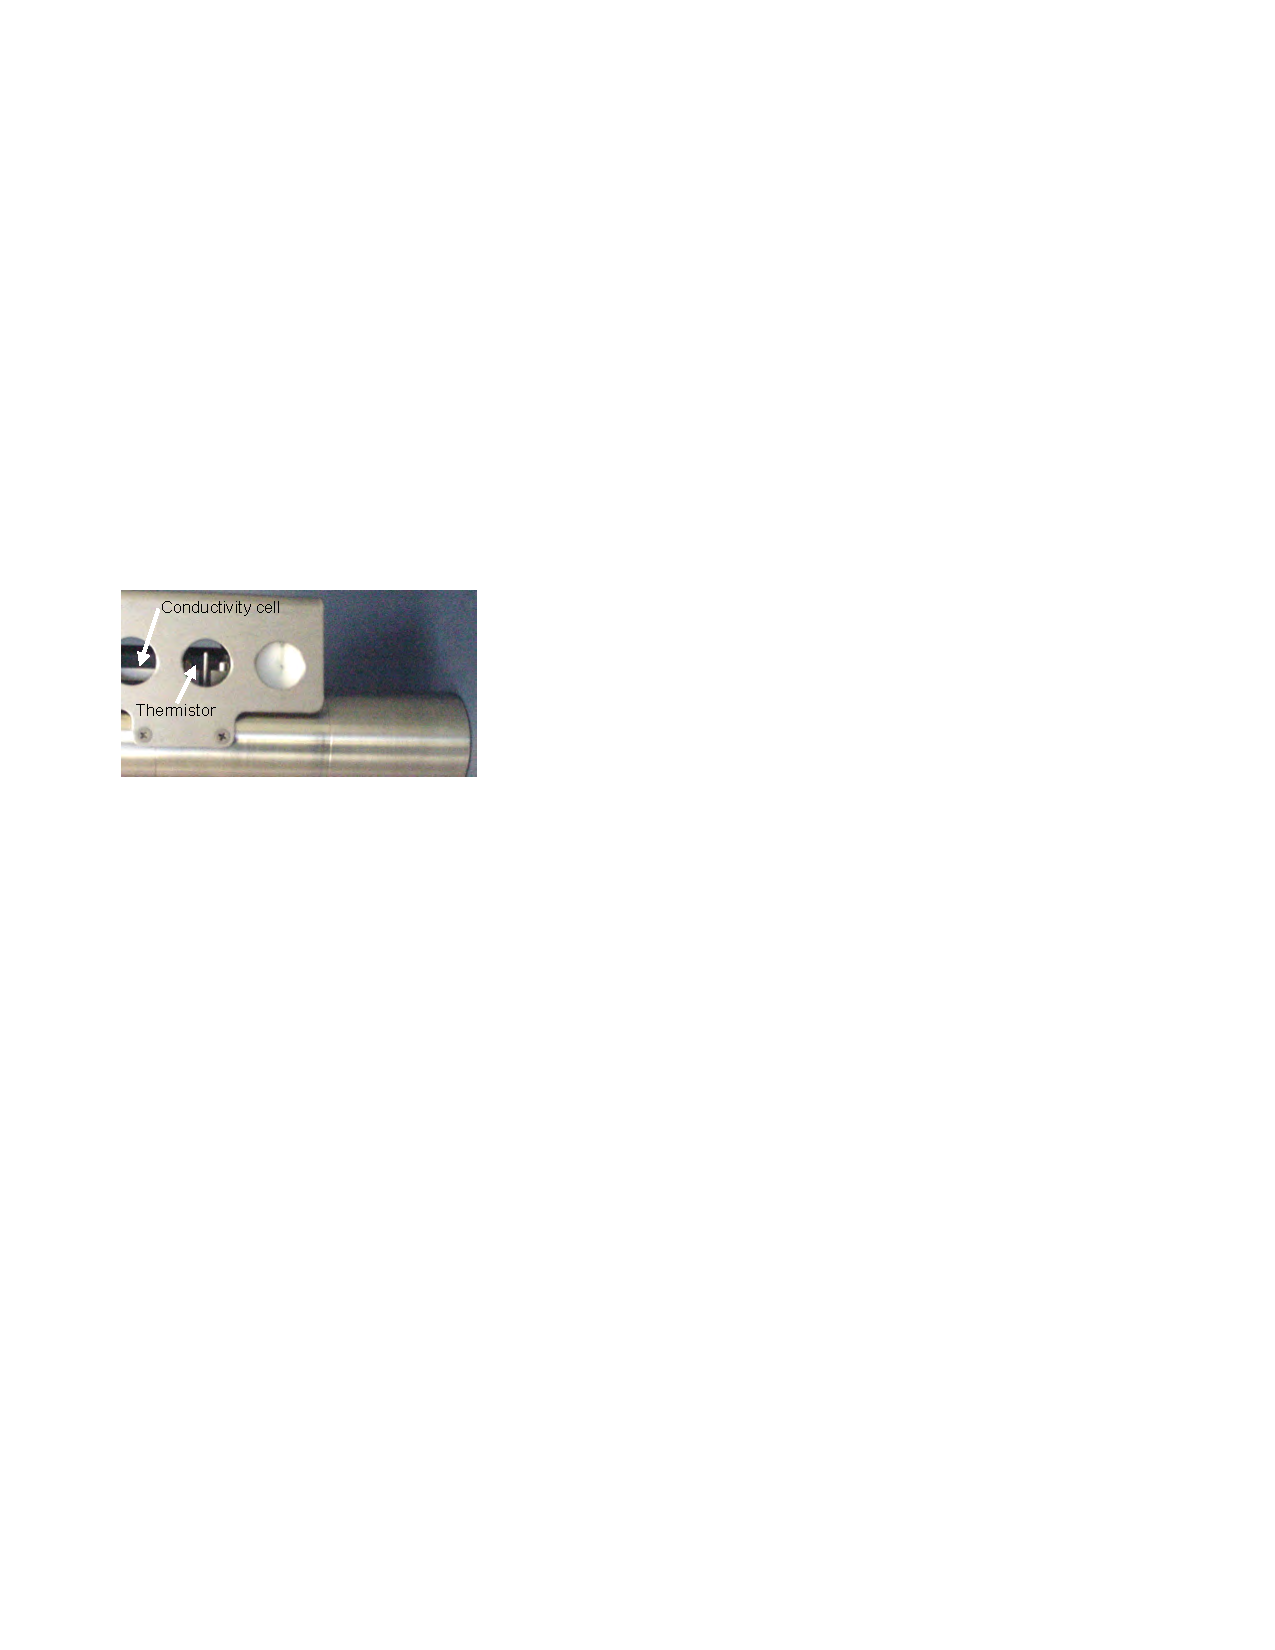
\includegraphics[width=3in]{figs/ThermistorConductity.pdf}
    \caption{a) CTD b) thermistor and conductivity probe on a CTD.}
    \label{fig:CTD}  
  \end{center}
\end{figure}

Temperature is measured in the ocean by thermometers.  The typical technology is what is called a ``\Wikiref{thermistor}'', which is a metal in which the electrical resistance changes proportional to its temperature.  Since its relatively easy to design an electronic circuit to measure resistance, this has allowed rapid and automatic measurement of ocean temperatures since such thermistors were first developed in the 1970s.  

Once calibrated, quality ocean thermistors are typically accurate to $0.001\ ^oC$, and are stable to similar levels. It takes time for the thermistor to respond to temperature changes in the ocean, so designing the sensors is a tradeoff between physical robustness and response time.  Typical response time is about 0.3--0.5 s, which is quite fast for ocean changes, but can be slow relative to a CTD being lowered in the ocean. 

\subsection{In-situ and potential temperature}
\label{sec:potential-temperature}

Ocean temperatures are largely set at the sea surface either by absorbing sunlight or exchanging heat with the atmosphere, and subsequently modified by ocean mixing.  The temperature of the water is thus a powerful \emph{tracer} of where a water mass last saw the surface of the ocean, with warmer waters found near the equator, and colder near the poles.    


However, the effect of pressure on the temperature makes it harder to trace where water came from.  The temperature of a water parcel that is moved from one depth to a deeper one will increase because the pressure has increased, even if no heat is exchanged with its surroundings during the move (we call this an \emph{\Wikiref{adiabatic process}}).  A thermistor will measure this change. If the parcel is \emph{adiabatically} brought back to the original depth, its temperature will drop again.  

In order to remove this adiabatic heating effect, its useful to differentiate between the actual \emph{in-situ} temperature and instead report the \emph{potential temperature}.  This is simply the temperature the water would be if it was brought adiabatically to the surface.  

The reason for doing this is dramatically illustrated by considering the temperature measured in the Kermadec Trench \citep{Warren73}.  The trench is much deeper than the surrounding water, so water in the trench has been there a long time.  However, the in-situ temperature increases with depth which might make us think either it is different water, or that there is a heating source from below (\fref{fig:Trench}, curve labeled with "t").  However, computing the \emph{potential temperature} $\theta$ shows that this water is the same potential temperature (\emph{isothermal}) deeper than 5000 m.   

\begin{marginfigure}
\begin{center}
  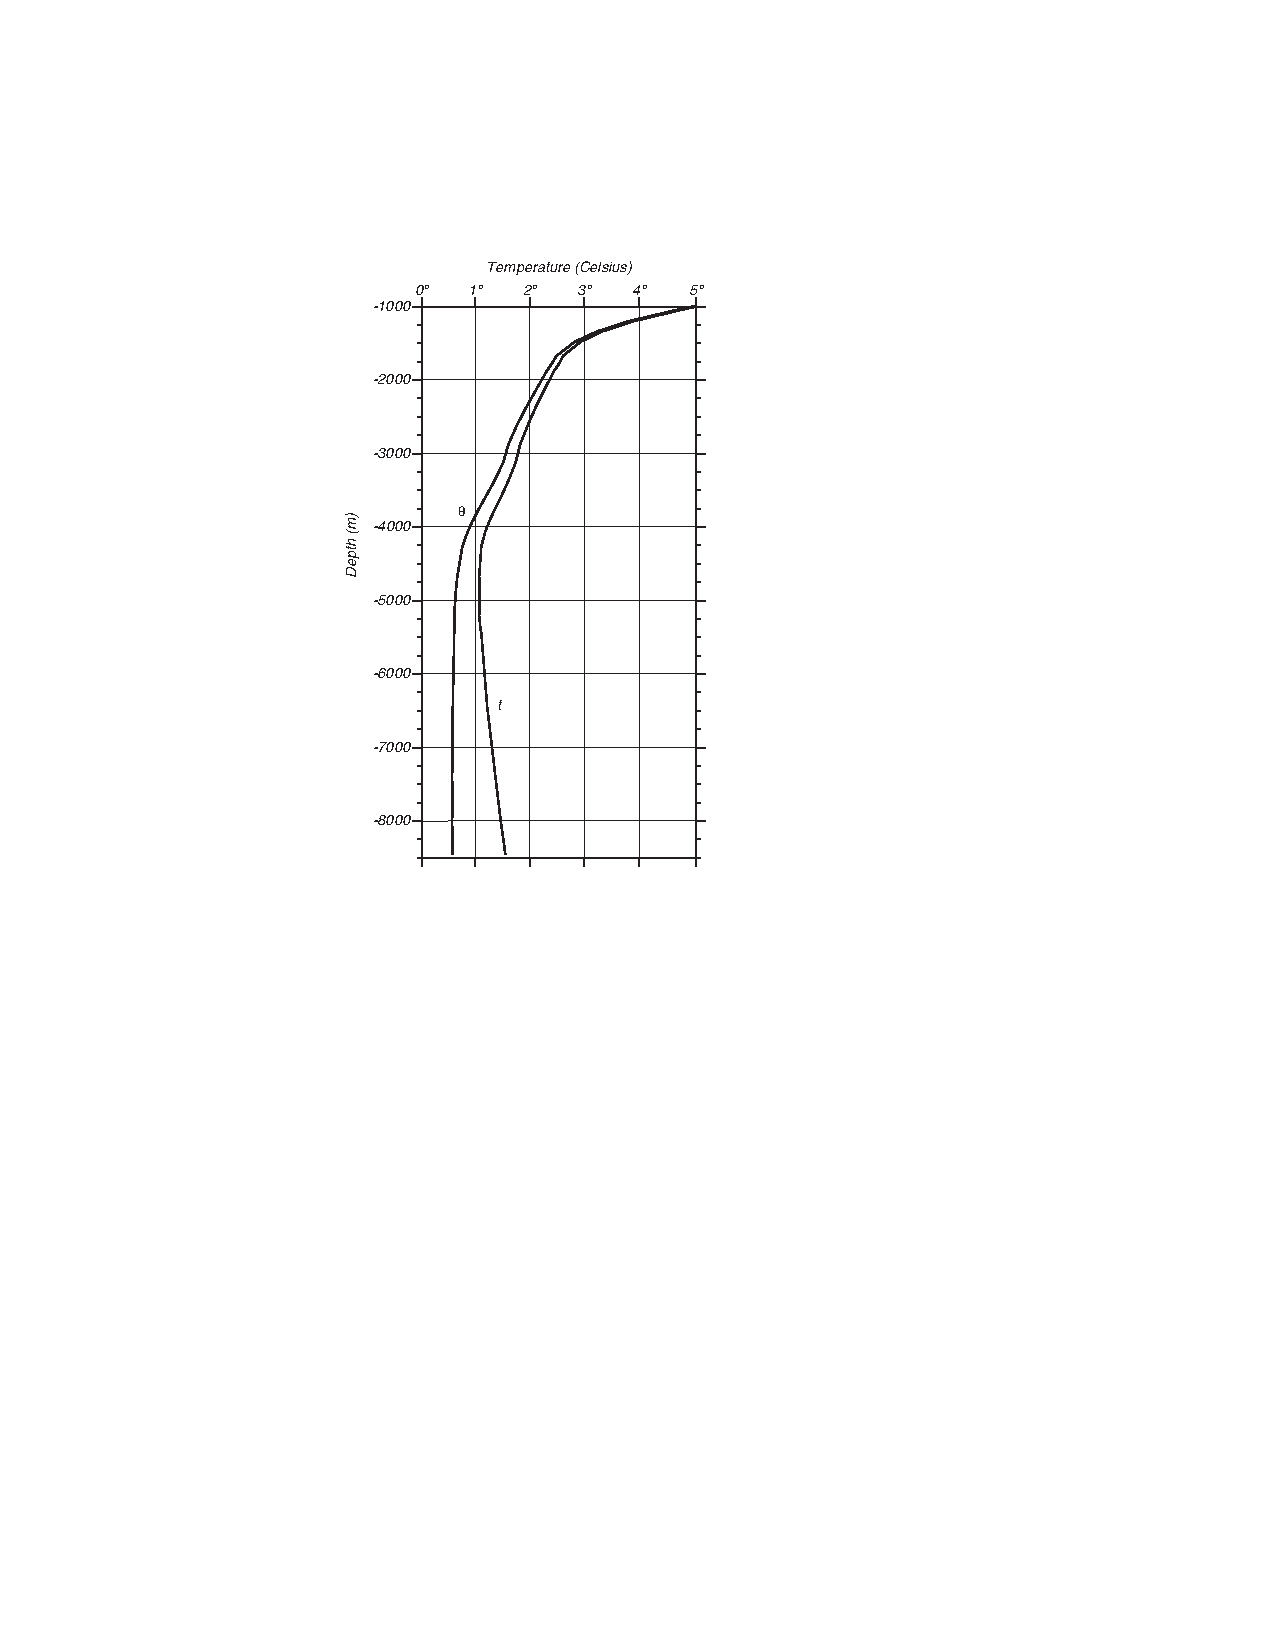
\includegraphics[width=2in]{figs/Trench}
  \caption{CTD data from Kermadec Trench \citep{Warren73} \emph{in situ} temperature and potential temperature. (Figure from \href{http://oaktrust.library.tamu.edu/handle/1969.1/160216}{Stewart})}
  \label{fig:Trench}
  \end{center}
\end{marginfigure}

Outside of the deepest part of the ocean, the difference between potential and in-situ temperatures are not large (\fref{fig:P16Temp}).  In the deepest ocean, its clear that the cold tongue of water that originates in the Antarctic Circumpolar Current originates shallower in the water column than we would infer from just looking at the \emph{in-situ} temperature.  This improved ability to trace the source of water without accounting for pressure effects is the main motivation for using potential temperature, and most publications will use potential temperature exclusively.  

\begin{figure}[hbt]
  \begin{center}
    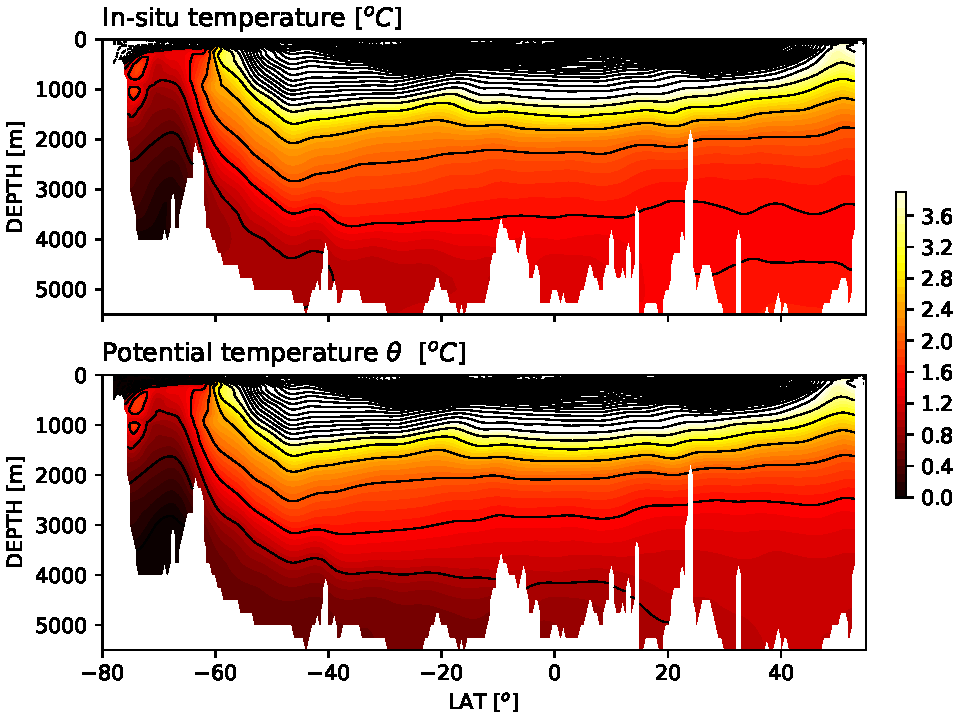
\includegraphics[width=5in]{./figs/P16Temp.pdf}
    \caption{North-south sections in the Pacific ocean at a longitude of 150 W, plotted as the measured \emph{in-situ} temperature (upper panel) and the potential temperature, $\theta$ (lower panel).    }
    \label{fig:P16Temp}  
  \end{center}
\end{figure}

\section{Salinity}

Salinity is the measure of dissolved solids in seawater, and is expressed as grams of solids per kilogram of seawater.  Because it is derived from solids in the seawater, salinity is hard to define, and quite hard to accurately measure in the ocean. Oceanographers are greatly aided by the fact that the residence time of a salt ion is very long compared to the mixing timescale of the ocean.  While we think of rivers as being composed of fresh water, the input of salt ions largely come from the trace amounts in these rivers. In total, there is $\approx 5 \times  10^{19}\ kg$ of salt in the ocean, but inputs are $\approx 2.5 \times  10^{12}\ kg/year$, so the \emph{\Wikiref{residence time}} of salt in the ocean is around 20 million years.  The overturning time scale of the ocean is 3000 y (at the most), so salt in the ocean is ``well-mixed''. This long residence time means that the ratio of salt constituents in the oceans only changes on geological time scales, and thus in the open ocean the ratio of various ions can be considered a constant (closer to river sources the ion ratios can be quite different).  

Note, however, that the ratio of the solids that make up the salt being constant does not mean that \emph{salinity} itself is constant.  The concentration of salt in a given volume of water depends on how much river water or rain water that parcel has been in contact with, or if it has been subject to evaporation.  

\subsection{Measurement}

Chemical oceanographers spent many decades studying the chemical makeup of salt water.  The standard way of measuring salinity was to titrate the chloride solids and then use the fact that the ratio of salt ions in the ocean is relatively constant to infer the total salinity.  This is done more rarely now, and instead oceanographers measure the \emph{conductivity} of  seawater using a conductivity cell. This uses the fact that salt water conducts electricity better than fresh water, and thus the amount of electricity thats able to get from an electrode to an anode through a known quantity of seawater is proportional to the conductivity. 

Electric circuits to measure conductivity are relatively straight forward, but the most stable measurements require a good-sized sensing sensing element over which to take the measurement.  The conductivity cell in the CTD shown in \fref{fig:CTD}a is about 15 cm long to allow a stable and accurate estimate.  This means that there is a limitation to how fine the vertical resolution of the conductivity estimate is.

\begin{marginfigure}
\begin{center}
    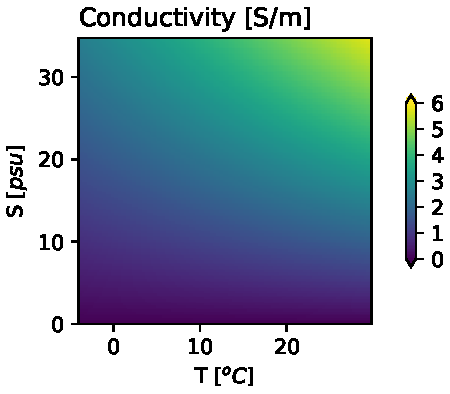
\includegraphics[width=2.2in]{./figs/Conductivity}
    \caption{Conductivity as a function of temperature and salinity}
    \label{fig:Conductivity}
\end{center}
\end{marginfigure}

The largest challenge in measuring salinity using conductivity is that conductivity is also a strong function of temperature as well as salinity (\fref{fig:Conductivity}).  That means that we need to have a well-matched temperature measurement at the same time and place as the conductivity measurement in order to back out the salinity.  Mismatched sensors lead to a phenomena known as "salinity spiking".  It is easily understood if we consider measuring through a temperature interface in water that  has a uniform salinity (\fref{fig:SalinitySpike}).  If the temperature sensor is lagged compared to the the conductivity sensor, the conductivity will go down, but the temperature measured by the temperature sensor will not until a deeper depth.  When the salinity is calculated from these two measurements, there will be a sharp discontinuity in inferred salinity at the interface because the sensors are not matched up. This is a very hard problem to get rid of, and involves making sure the two sensors are not lagged from one another, and making sure that their signals are smoothed enough that the mismatch in how the sensors respond to changes are smoothed over.  

\begin{figure}[hbt]
  \begin{center}
    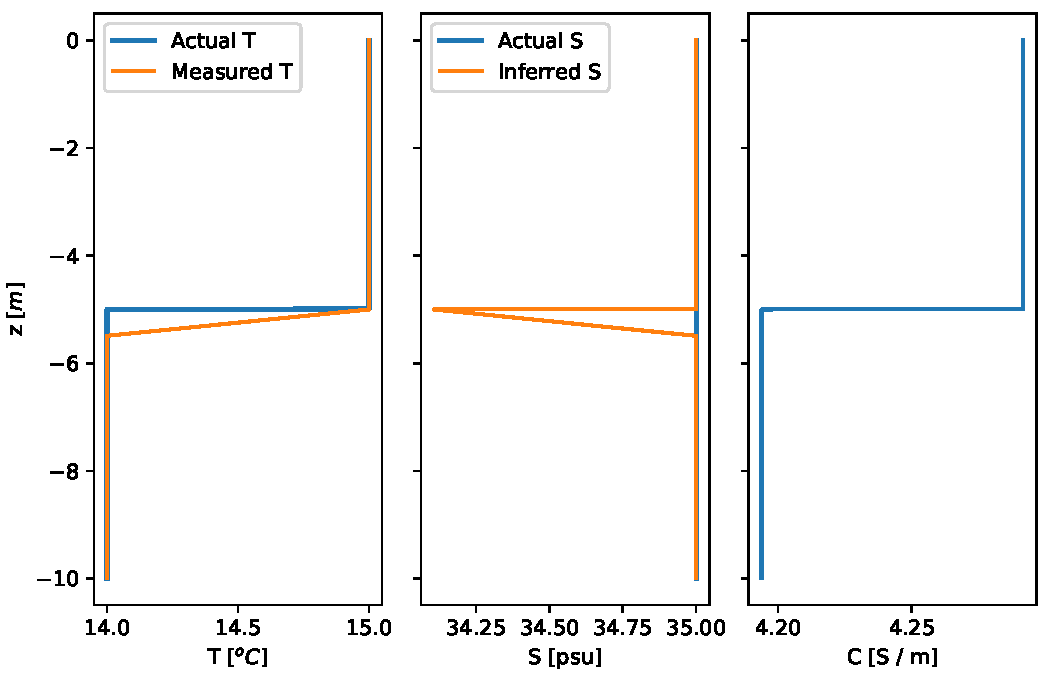
\includegraphics[width=4in]{./figs/SalinitySpike.pdf}
    \caption{Salinity spiking due to conductivity and temperature sensors not being aligned; here the temperature sensor lags the conductivity sensor, so the cold change with depth is registered in the conductivitsy sensor before the temperature. Note the conductivity change is completely due to temperature.}
    \label{fig:SalinitySpike}
  \end{center}
\end{figure}

Regardless of measurement issues, the measurement of salinity using conductivity and temperature is very wide spread.  In order to differentiate such measurements from fundamental chemically based estimates, oceanographers often use the units of "practical salinity units" or "psu".  When these units are used, the measurement is almost always from a CTD.  More recently, there is a new salinity unit used as part of an update to the equation of state (\href{www.teos-10.org}{TEOS10}), where salinity is denoted as "absolute salinity" (AS), and the units are g/kg.  For this class we will use the older ``psu''a.   

\section{Pressure}
\label{sec:pressure}

Pressure is the force per unit area that a parcel of fluid exerts on its neighbours.  Remember that in a fluid (gas or liquid), the molecules are in free motion.  As discussed above, the more kinetic energy in this motion, the higher the temperature of the fluid.  That same kinetic energy exerts itself as a force on any container that holds the molecules. Consider a ballon filled with air.  The air inside the balloon is pushing out against the ballon with a certain force per area.  This happens because the molecules of air are moving in random motion due to their heat, and some of that momentum is exerted against the balloon's surface.  Force always has a direction, but pressure forces are omni-directional or \emph{isotropic}.  So in the case of the balloon, the force exerted by the pressure is always perpendicular to the surface of the balloon.

\begin{figure}[h]
    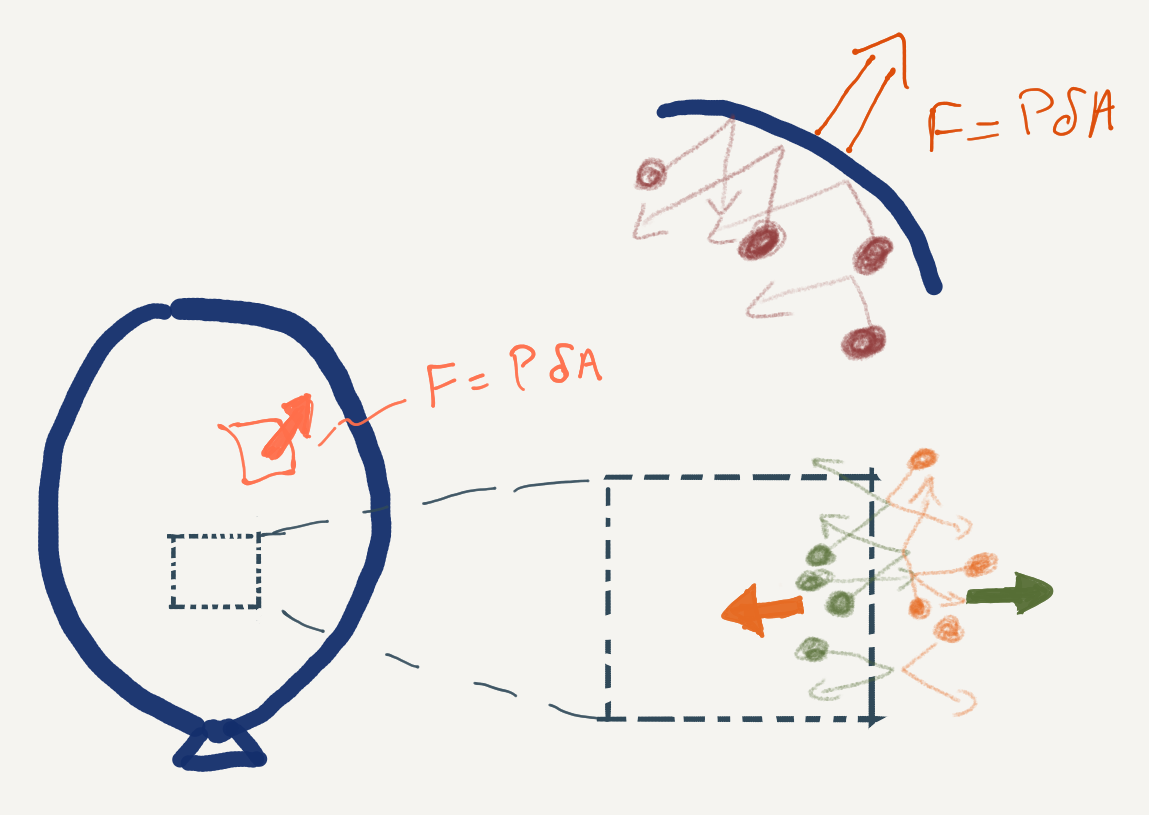
\includegraphics[width=2.8in]{figs/Balloon.png}
    \caption{Sketch of how molecules in a fluid exert pressure on a balloon and on one another. First blowup is a schematic of air molecules hitting the balloon, second is of molecules on one side of a surface inside the air hitting molecules from the other side and the two sets of molecules therefore exerting a force on one another.  Note that in order to get a force we must specify an area element, which we've called $\delta A$ here.  }
    \label{fig:Ballon}
\end{figure}

Inside the balloon, the molecules  exert a pressure force on one another. If we insert an area element somewhere in the balloon, the molecules on the left side of the barrier exert a force to the right, and the molecules on the right side exert a force to the left.  If the pressure is the same on both sides of the area element, then the forces are equal and opposite and the fluid will be stationary.  If there are \emph{pressure gradients} inside the balloon, then one side may push harder than the other and the fluid will move.  We discuss pressure gradients a great deal in this class and will come back to them below (\fref{sec:pressure-gradients}).  

\subsection{Measuring pressure}

This is usually relatively straight forward using a \href{https://en.wikipedia.org/wiki/Strain_gauge}{strain gauge}.  The CTD is equipped with a pressure gauge that is typically sensitive to better than .0025\% of their range.  Hence a deep-ocean pressure sensor capable of measuring to 7000 m will have an accuracy of 0.14 dbar.  

The units of pressure are ``officially'' Pascals, with $1\ Pa = 1\ N\,m^{-2}$.  However, oceanographers almost always  report in the units of ``decibars'', where $1\ Pa = 10^{-4}\ dbar$.  The reasoning behind this is straight forward: pressure at 1-m depth is $g \rho_0 \Delta z = 9.8 \times 1023 \times 1 = 10025\ Pa = 1.0025\ dbar$.  So the pressure at a depth of 1-m is very close to 1 dbar.  



\section{Calculating density}

Density is the mass per volume of a substance, and expressed in $\mathrm{kg\ m^{-3}}$.  The density of seawater varies from approximately $1000\ \mathrm{kg\ m^{-3}}$ for freshwater near the surface at 4 degrees C, to $1050\ \mathrm{kg\ m^{-3}}$ in the very deepest ocean, at salinities of 35 psu, temperature $-1\ \mathrm{^oC}$ and at a depth of 5000 m.  Notable is the fact that density of seawater only varies by about 5\% over the world's oceans.  

Density differences in seawater give rise to pressure differences, and hence help drive currents in the ocean; less dense water wants to float on top of more-dense water (for example in \fref{fig:lock-exchange}) .  Unfortunately, there is no direct way to measure density \emph{in-situ}, and scooping volumes of water out of the ocean to weigh is highly impractical.

\begin{figure}[htbp]
    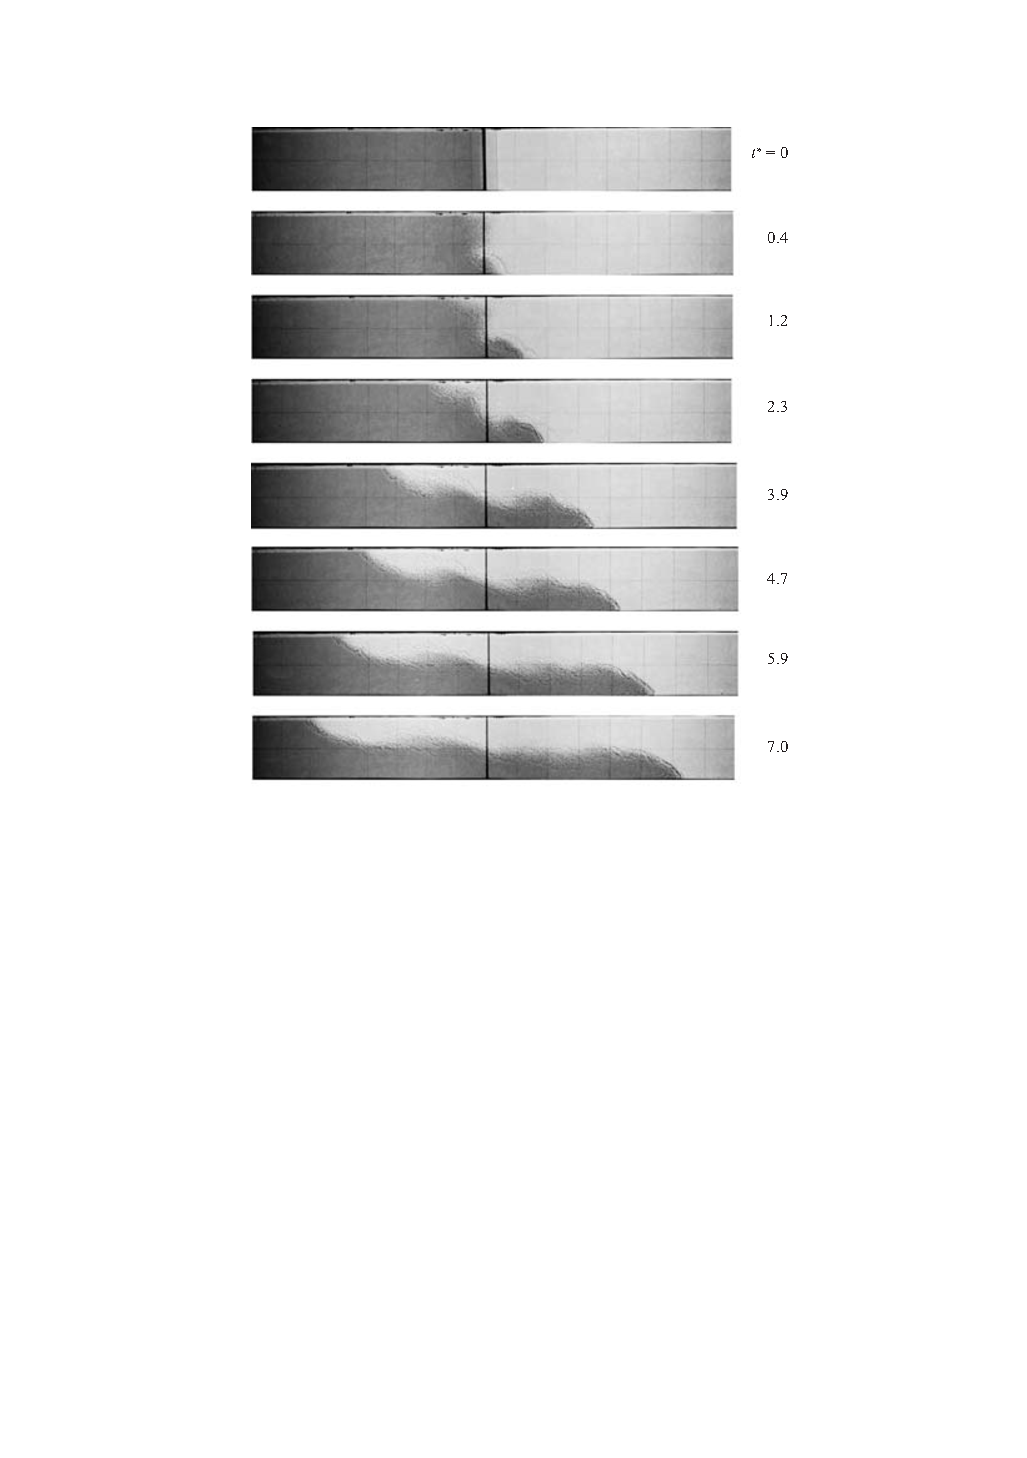
\includegraphics[width=3in]{./figs/ShinEtAl04Fig2.pdf}
    \caption{Lock exchange with dense water on left and light water on the right. \citep{Shinetal04}}
     \label{fig:lock-exchange}  
\end{figure}

Instead, we rely on \emph{empirical} relationships between density and the ``state'' of the seawater.  The state variables that give the density are  temperature, salinity, and pressure.  Increasing the temperature of water tends to decrease the density (except near the freezing point), while increasing the salinity and pressure tend to increase the density.  

\subsection{Density relation}


\begin{marginfigure}
    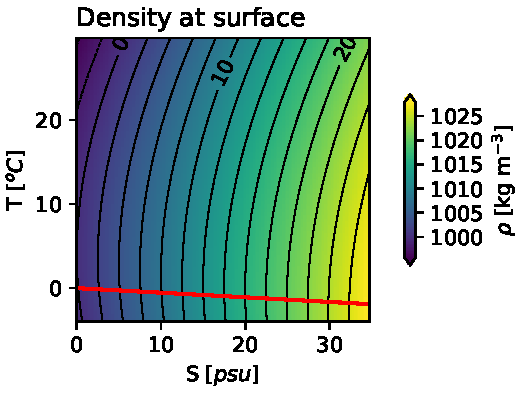
\includegraphics[width=2.7in]{./figs/Density.pdf}
    \caption{Density as a function of T and S at the sea-surface.  Contours are the density, the red line is the freezing point at the sea surface.  }
    \label{fig:Density}  
\end{marginfigure}

The equation for density is a non-linear function of temperature, salinity, and pressure, and is determined empirically.  Various equations of state have been published over the years, but the typically used ones are EOS80 and TEOS-10.  See the \href{http://www.teos-10.org}{TEOS-10} website for details and references.  The differences between these are subtle, and for our purposes we will use the older EOS80.  

The non-linearity of the equation of state is clear in \fref{fig:Density}.  For a given salinity, the density depends on the temperature in a non-linear fashion, with density changing more quickly with temperature at high temperatures and more slowly at low temperatures, and indeed changing sign at the lowest temperatures, with density dropping again as temperatures get lower.  Practically, this means that we must compute the density of seawater on a computer; there are specialized software packages to do this (\texttt{seawater} and/or \texttt{gsw} routines in Matlab, python, or R).

Often, however, it is useful to \emph{linearize} the equation of state if T, S, and P do not vary much.  In that case we can write:

\begin{eqnarray*}
    \rho & \approx & \rho_0 \left[ 1 - \alpha \left(T - T_0\right) + \beta \left(S - S_0\right) + \gamma \left(P - P_0\right)\right]\\
    \Delta \rho & \approx & \rho_0\left[- \alpha \Delta T + \beta \Delta S + \gamma \Delta P\right]
\end{eqnarray*}

$\alpha$ is called the ``thermal expansion'' co-efficient, and for values  $T_0, S_0, P_0 = 15, 30, 0$ is $\alpha \approx 2\times 10^{-4}\ \mathrm{[^oC^{-1}]}$; so for a change of temperature of $+1\ ^oC$ the density decreases $0.2 \ \mathrm{kg\, m^{-3}}$.  At the same values, $\beta \approx 7\times10^{-4}\ \mathrm{psu^{-1}}$, so a change of 1 psu increases the density by $0.7 \ \mathrm{kg\, m^{-3}}$.  For the same values the value of $\gamma \approx 4.5\times10^{-6} \ \mathrm{dbar^{-1}}$, so moving a parcel 1 dbar higher pressure will increase its density by $+4.5\ \times 10^{-3} \ \mathrm{kg\, m^{-3}}$.  Note that $\gamma$ is relatively linear, so moving to 1000 dbar (i.e. 1000-m deep) increases the density by $+4.42\ \mathrm{kg\, m^{-3}}$.   

\subsection{Potential density}
\label{sec:potential-density}

\begin{figure}[hbt]
  \begin{center}
    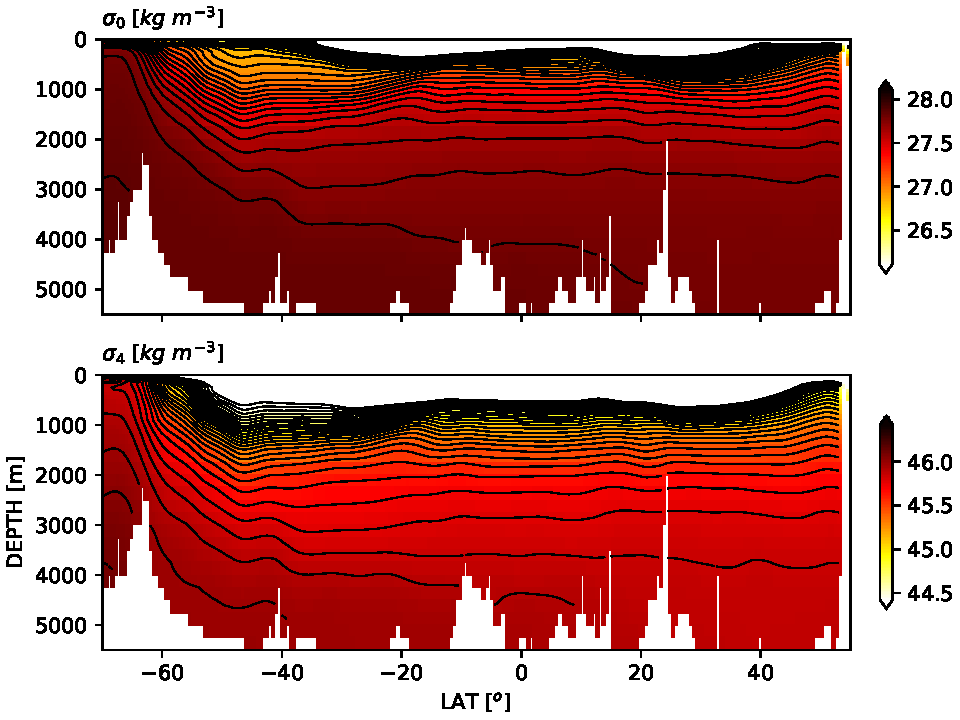
\includegraphics[width=4.5in]{figs/P16Pden.pdf}
    \caption{Potential density along P16 hydrographic section (north-south along approximately 150 W) relative to the sea surface (top plot) and relative to 4000 dbar (bottom plot).  Both are contoured with the same-spaced contour intervals, though the absolute values are different.  Note some near-surface contours have been omitted for clarity.}
    \label{fig:P16Pden}  
  \end{center}
\end{figure}

The concept of potential density is similar to that of potential temperature (\fref{sec:potential-temperature}), where we would like to remove the pressure effect from the density in order to see where a parcel of water originated.  Unfortunately, the non-linearity of the equation of state of seawater makes it impossible to do this cleanly, in that if we change the pressure at one depth, the change of density is not the same if we change it at another depth $\Delta \rho(S, T, \Delta P, P=0) \neq \Delta \rho(S, T, \Delta P, P=4000)$.  For $S=30\ \mathrm{psu}$, $T=15\ \mathrm{^oC}$, $\Delta P = 10\ \mathrm{dbar}$ we have $0.0447\ \mathrm{kg\ m^{-3}}$ at 0 dbar, and  $0.0412\ \mathrm{kg\ m^{-3}}$  at 4000 dbar.  To deal with this, we calculate the ``potential density'' relative to a given pressure.  

The most commonly used potential density is calculated relative to  the surface pressure and is signified as $\sigma_{\theta} = \rho(S, T, 0) - 1000\ \mathrm{kg\ m^{-3}}$.  Note subtracting 1000 from the density is because all ocean densities are near 1000.  Often seen are potential densities relative to 1000-m depth increments in the ocean, signified at $\sigma_1, \sigma_2, \sigma_3, \sigma_4$.  Each gives a  different view of the density along P16 (\fref{fig:P16Pden}).  If we adiabatically bring the deep water to the surface it all appears almost the same density, whereas if we bring it to 4000 m there is much more apparent ``stratification'' (more contour lines per depth).  If we are interested in the dynamics of the deep sea, these adjustments are crucial.  

The contours of potential density in \fref{fig:P16Pden} are called ``isopycnals''.  

As a vivid example of how the equation of state depends on both temperature and salinity, again consider the section along P16 in the Pacific (\fref{fig:P16PdenwTS}).  The potential temperature and salinity is contoured with potential density contours.  It is clear that water at a given density is colder and fresher as you move north, and hence both temperature and salinity are necessary to understand the density of the ocean.  

\begin{figure}[hbt]
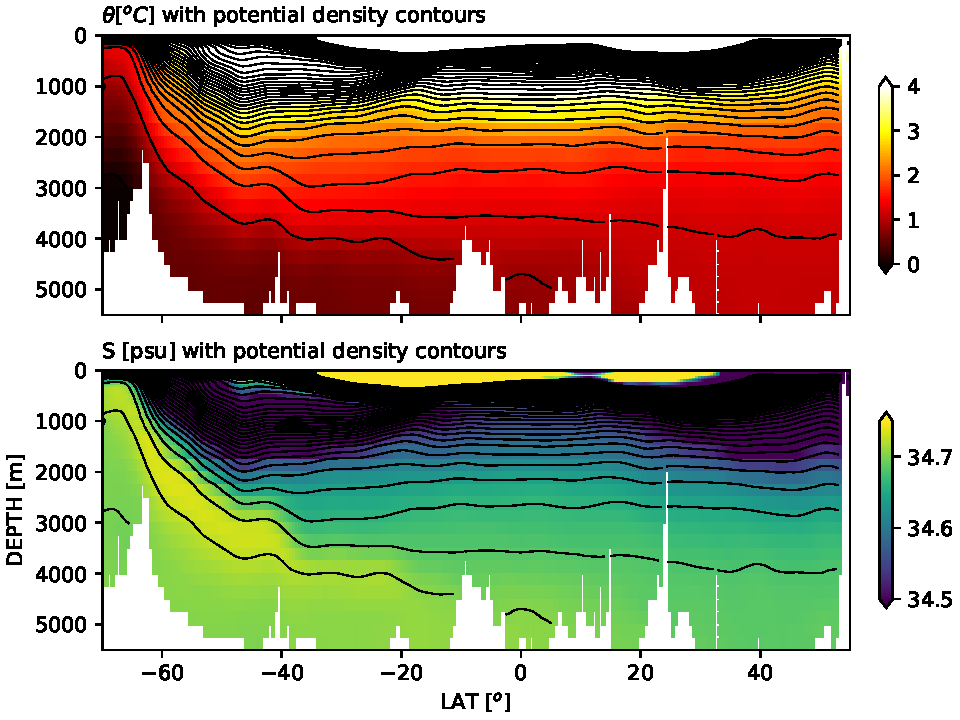
\includegraphics[width=4.5in]{./figs/P16PdenwTS.pdf}
\caption{Potential temperature and salinity contoured with isopycnals anlong section P16 in the Pacific Ocean}
\label{fig:P16PdenwTS}      
\end{figure}

Another way of looking at the same data that we will use a lot in this course is to plot the data in $\theta-S$ space, where each dot is a separate measurement of temperature and salinity (\fref{fig:P16TSzoom}).  The red data dots are in the south, and blue in the north, and along most isopycnals, the water becomes fresher and colder as profiles from progressively further north are looked at.

\begin{figure}[hbt]
    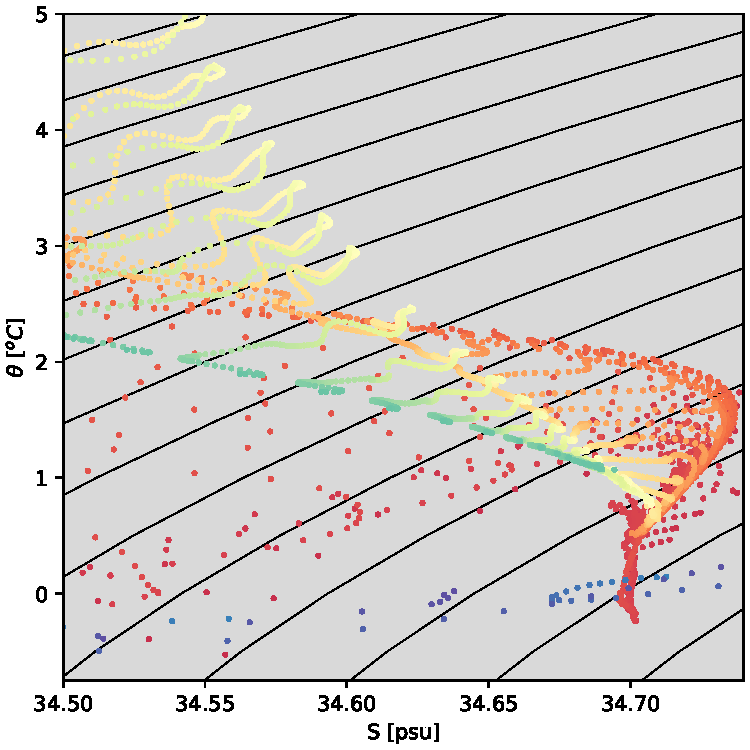
\includegraphics[width=3.0in]{./figs/P16TSzoom}
    \caption{Potential temperature as a function of Salinity along P16. Red data points were collected in the south, and blue data points in the north.  Isopycnals (relative to atmospheric pressure) are contoured.  Note only water below 1000-m is shown here.}  
    \label{fig:P16TSzoom}
\end{figure}

\subsection{Cabbeling}

\begin{marginfigure}
    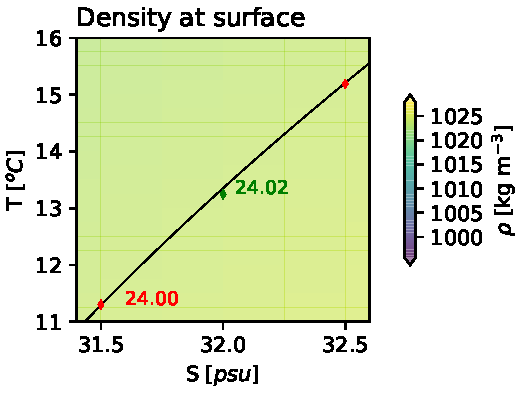
\includegraphics[width=2.5in]{./figs/Cabelling.pdf}
    \caption{Density as a function of T and S at the sea-surface.  Contours are the density, the red line is the freezing point at the sea surface.  }
    \label{fig:Cabelling}  
\end{marginfigure}

A final note about the equation of state of seawater is the curious effect known as \Wikiref{cabbeling}. As we will discuss in this course, mixing waters of different densities requires energy to overcome the density differences between the water masses.  Therefore water tends to be relatively sorted with depth, with dense water under light.  However, there exist substantial temperature-salinity (T/S) differences in the ocean, and as we can see from \fref{fig:Density} there is a whole range of T/S properties for any one density contour. It requires very little energy to mix two water parcels on the same \emph{isopycnal}.

However, if we mix two water masses from the same isopycnal, throughout most of the ocean it will lead to a new, slightly denser water mass, as illustrated \fref{fig:Cabelling}.  If equal volumes of water masses with T/S properties signified by the red dots along the $\sigma_{\theta} = 24\ \mathrm{kg\,m^{-3}}$ isopycnal are mixed, their T/S properties fall exactly half way between the parents (green dot). But a water mass with those T/S properties has a density of $\sigma_{\theta} = 24.022\ \mathrm{kg\,m^{-3}}$, which is a bit denser than the parent water masses.  This curious effect is believed to cause circulation in the ocean, particularly near sharp fronts and at high latitudes where the effect is most pronounced.   

\section{Other seawater properties}

The properties described above are the main ones dealt with in this course, but there are a few others that are important.  

\subsection{Sound}

Sound speed in the water depends on its state variables (S, T, and P), and again can be looked up in empirical fits, typically ranging between 1450 and 1550 m/s (\fref{fig:SoundSpeed}), with higher speeds for warmer and saltier water.

 \begin{marginfigure}
 \begin{center}
    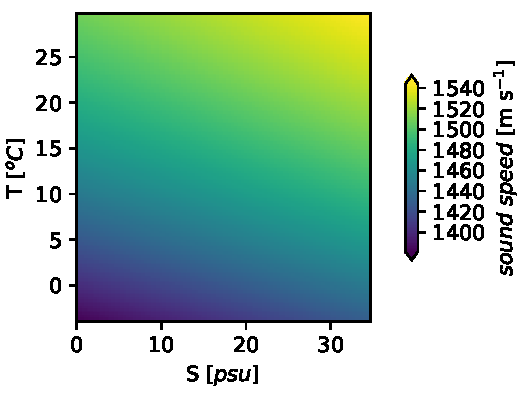
\includegraphics[width=2.5in]{./figs/SoundSpeed.pdf}
    \caption{Speed of sound in waters as a function of T and S at the sea-surface. }
    \label{fig:SoundSpeed}  
 \end{center}
\end{marginfigure}

Sound decays in seawater more slowly than in air, with higher frequency sounds decaying over shorter distances.  Sound also tends to spread spherically, so its energy falls off with the cube of the distance from the source (i.e. $r^{-3}$).  However, a peculiarity of the sound profile in the ocean means that there is a minimum in the sound speed approximately 500-1000 m deep in the ocean.  This occurs because sounds speed drops with temperature in the upper kilometer of the ocean, but increases with pressure in the bottom kilometer, where the temperature doesn't change very quickly \fref{fig:sofar}.  This minimum in the sound speed creates a (sound) waveguide called the \Wikiref{SOFAR} channel (Sound Fixing and Ranging).  Waves always refract towards a slower medium, so a sound emitted in the SOFAR channel will start to move upwards and downwards in the water column, but the waves (and hence sound energy) will be refracted back towards the SOFAR channel.  This means that instead of sound falling off as $r^{-3}$, it falls off as $r^{-2}$, which is much slower.  This effect makes it possible for submarines and whales to communicate over long distances using low-frequency sound.  

\begin{figure}[hbtp]
  \begin{center}
    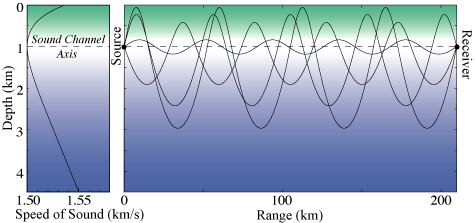
\includegraphics[width=4in]{./figs/sofar-color-big.png}
    \caption{Schematic of the SOFAR channel, left is sound speed profile, and on right are sound rays sketched from a source in the SOFAR channel (from \href{https://dosits.org/science/movement/sofar-channel/}{Sound in the Sea}) }
    \label{fig:sofar}
  \end{center}
\end{figure}

\subsection{Light transmission}


While sound can propagate long distances in the ocean, light cannot.  In clear water, less than 10\% of incoming light penetrates deeper than 50 m (\fref{fig:Light-Intensity}), with blue light (short wavelengths) getting deeper than red light (long wavelengths). Note that the longer-wavelength red light decays the fastest, whereas longer wavelength sound waves decay more slowly.  Thats because the decay of light is due to absorption by the water molecules. 

\begin{marginfigure}
    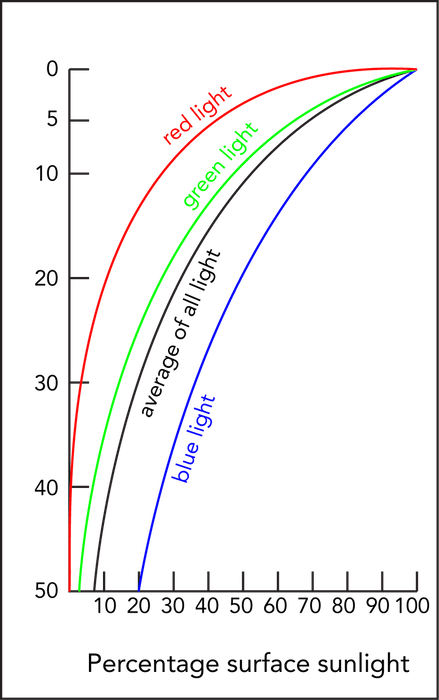
\includegraphics[width=2.0in]{figs/Light-Intensity.png}
    \caption{Profiles of light penetration in the ocean for different colors.  \href{https://manoa.hawaii.edu/exploringourfluidearth/media_colorbox/2788/media_original/en}{Inouye; Exploring Fluid Earth, U.\ Hawaii}}
    \label{fig:Light-Intensity}
\end{marginfigure}

The fact that light does not transmit very far in the ocean is an important difference with the atmosphere, where light is relatively transparent to air.  It means that radiative heat that comes in from the sun is mostly deposited in the upper few meters of the ocean, and we can think of it as deposited at the surface.  It also has profound effect on biological productivity of the ocean, since it means photosynthetic plant growth has to take place in the upper 10s of meters.  

\subsection{Ice}

The freezing point of water is indicated in \fref{fig:Density}, and is zero degrees for fresh water and decreases to less than zero for salty open-ocean water.  The effect of freezing ice on the ocean circulation is profound. Of course, locally it has the effect of insulating the ocean from the atmosphere.  Once ice forms on the surface, the loss of heat to the cold atmosphere drops precipitously, as any heat exchange has to propagate through the ice.  Further, the effects of wind on the ocean drop, as the wind has to move the more-solid ice floes around before it can have an effect on the ocean below.  Of course the ice floes do move, but the effect on the upper ocean is greatly dampened.  The wind also generates waves that can propagate under water (\emph{internal waves}), and these are greatly damped by ice cover.  Finally, ocean surface waves are radically damped, leading to a calmer sea state, and reduced \Wikiref{fetch (geography)} over which the waves can develop. 

The other very important effect of ice on the ocean is for deep- and bottom-water formation.  The densest waters in the ocean are formed near ice edges for two reasons.  The first is that these regions tend to be cold, and cold water is dense.  The second is that when ice freezes the salt crystals are not able to stay in the ice, a process known as \Wikiref{brine rejection}. The salt sinks away from the forming ice and is dissolved in the water underneath the ice-formation region leading to very cold and salty water.  This water sinks, and though it mixes as it goes, it remains dense enough to sink to the bottom of the ocean.  

\begin{figure}
       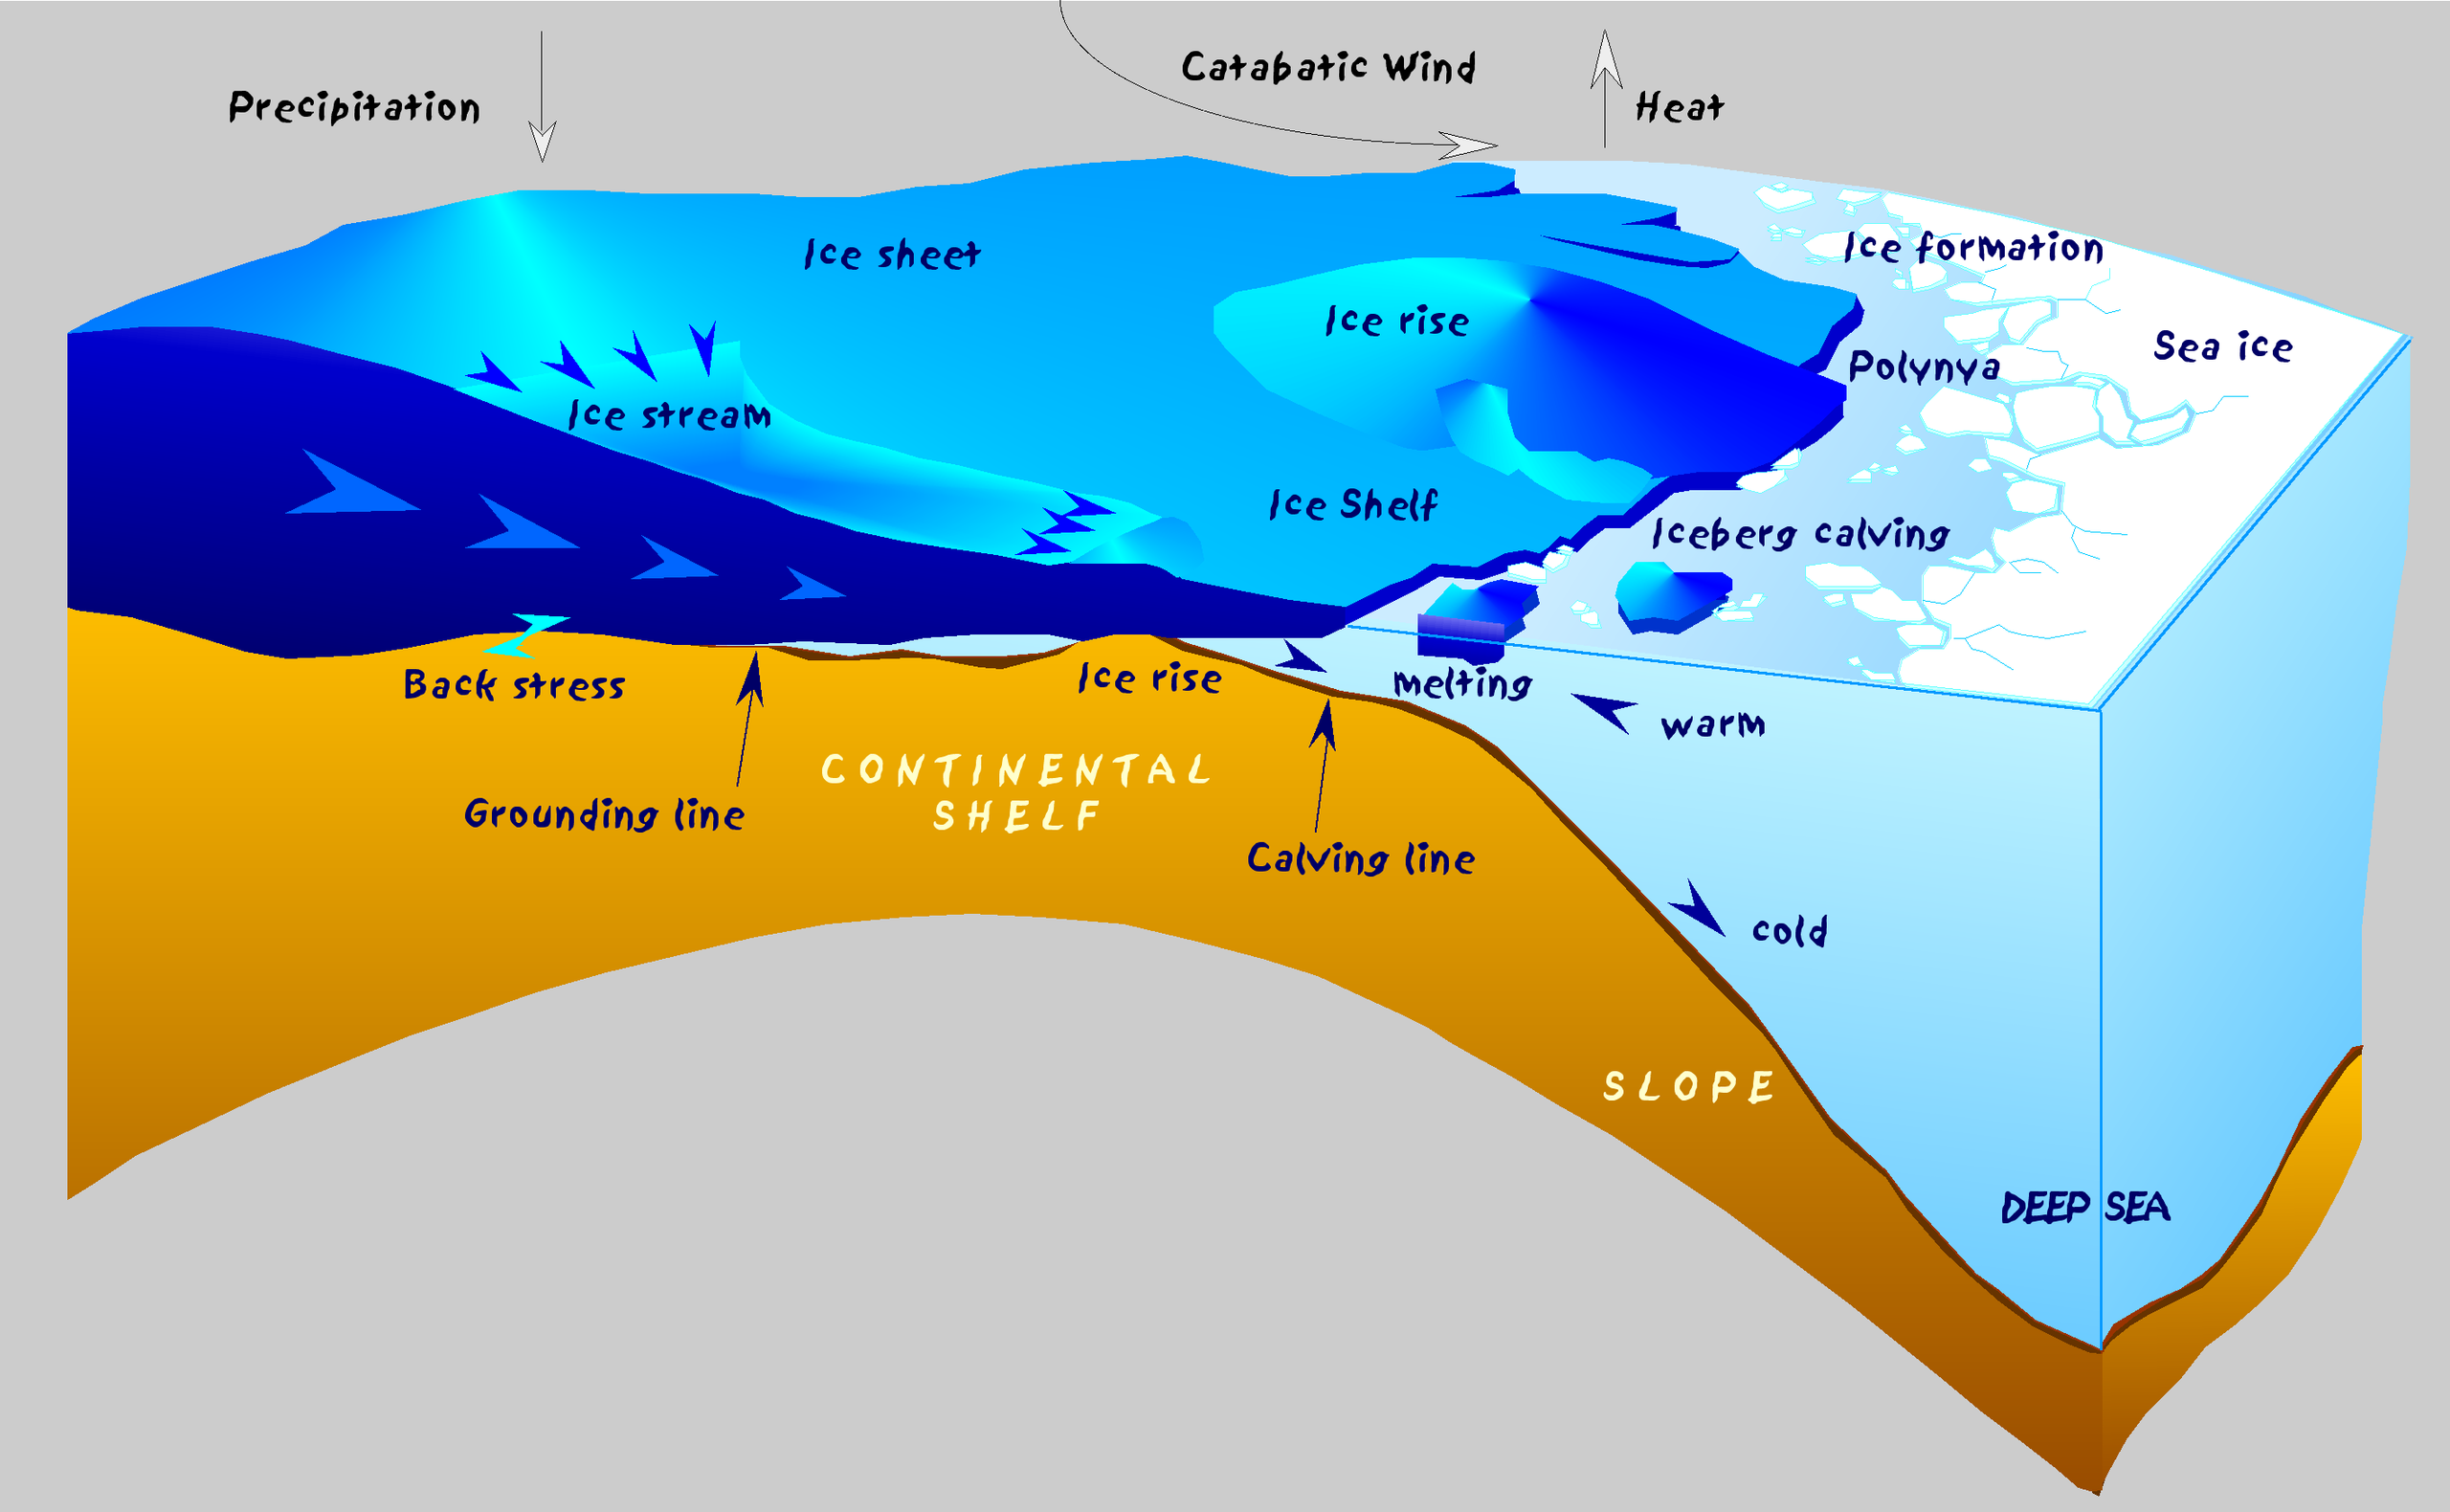
\includegraphics[width=3.2in]{figs/Antarctic_shelf_ice_hg} 
       \caption{Schematic of ice processes off the Antarctic continental shelf.  Catabatic winds blow off the continent and push the ice offshore.  New ice is formed, dense water produced by brine rejection and cooling, and the dense water sinks, bringing up new warm, fresher water from mid-depth. (From \href{https://en.wikipedia.org/wiki/Polynya}{Hannes Grobe, Alfred Wegener Institute for Polar and Marine Research, Bremerhaven, Germany})}
       \label{fig:AntarcticShelf}
\end{figure}

Deep-water formation tends to occur in ``marginal seas'' like the Wedell or Ross Seas off Antarctica, and the Greenland/Iceland seas in the north.  Dense water is produced in these regions at the ice edge, or in breaks in the ice forced by wind or by tidal mixing called \Wikiref{polynya}s. Polynyas tend to dominate the air-sea exchange of heat and brine production because they are open water but exposed to very cold and often windy conditions.  The wind forces the polynya to stay open by pushing ice downwind, but also drives dense water formation due to both brine rejection, sensible, and latent heat loss (\fref{fig:AntarcticShelf}).  This deep water forms \Wikiref{Antarctic bottom water} and \Wikiref{North Atlantic deep water} masses that can be traced throughout the world's oceans as anomalously cold and salty water;  the closer the water is observed to the source region, the colder and saltier it is.  This water can be clearly seen in T/S sections on the major ocean basins (\fref{fig:P16TempSalt}). We will discuss this substantially more in the next few weeks. 

\begin{figure}[hbt]
  \begin{center}
    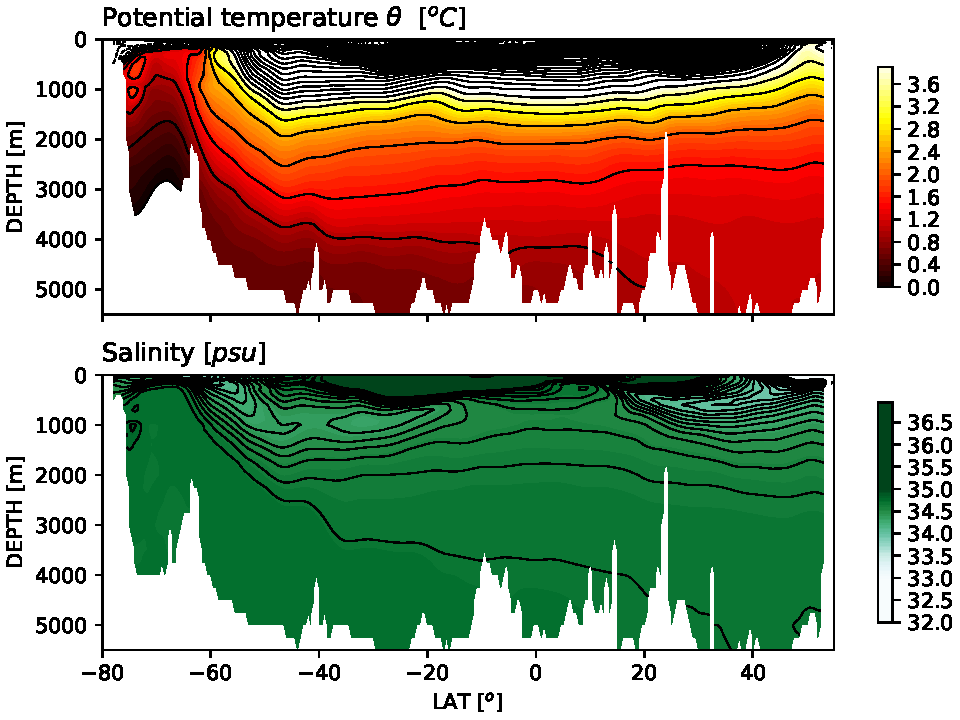
\includegraphics[width=4.5in]{./figs/P16TempSalt.pdf}
    \caption{North-south sections in the Pacific ocean at a longitude of 150 W of potential temperature, $\theta$ and salinity. Note the Antarctic bottom water starting south of -60 Lat, and pouring northwards into the Pacific.}
    \label{fig:P16TempSalt}  
  \end{center}
\end{figure}


%%%%%%%%%%%%%%%%%%%%%%%%%%%%%%%%%%%%%%%%%%%%%%%%%%%%%%%%%%%%%%%%%%%%%%
\chapter{Pressure Gradients}

Pressure is a very important quantity to the dynamics of the oceans,
and fluids in general.  Pressure \emph{gradients} give rise to net
accelerations that cause water to move, often in surprising ways.  There was some introduction to this qualitatively in the estuaries discussion.  Here we solidify those concepts quantitatively because we need to understand pressure gradients to make progress on understanding how the ocean moves.

\begin{figure}[htbp]
    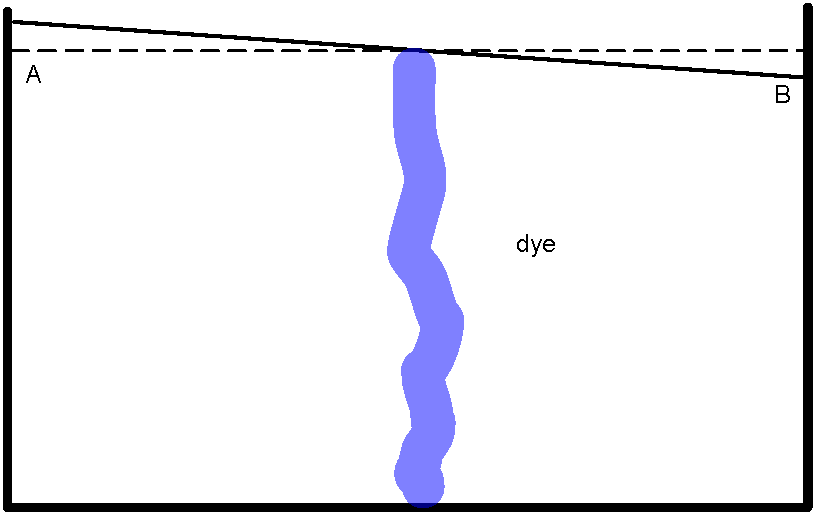
\includegraphics[width=3.5in]{./figs/PGFig1.pdf}
    \caption{A tank with the water surface tilted from equilibrium.  The surface wants to flatten, so water must be moved from area A to area B.  What is the action of a dye streak through the water column?}
    \label{fig:PGFig1}
\end{figure}

To motivate ourselves, recall the demo of sloshing water in a tank (\fref{fig:PGFig1}).  The surface interface is tilted such that area A is elevated, and area B is depressed.  Our intuition might say that the water needs to run downhill, and we may expect a flow, confined to the water surface, of water from area A to area B. Under this hypothesis, what do we expect the dye streak to do?  What does the dye stream actually do (approximately)?

To understand what is happening, we must understand pressure in the fluid.  The basic definition was given above (\fref{sec:pressure})


\section{Hydrostatic Pressure}

``Dynamic'' pressure happens for fast flows, like those over an
airplane wing.  Fortunately, in the ocean things are usually slow
enough that we can ignore the ``dynamic'' part, and focus on the
``hydrostatic'' part.

\begin{figure}[htbp]
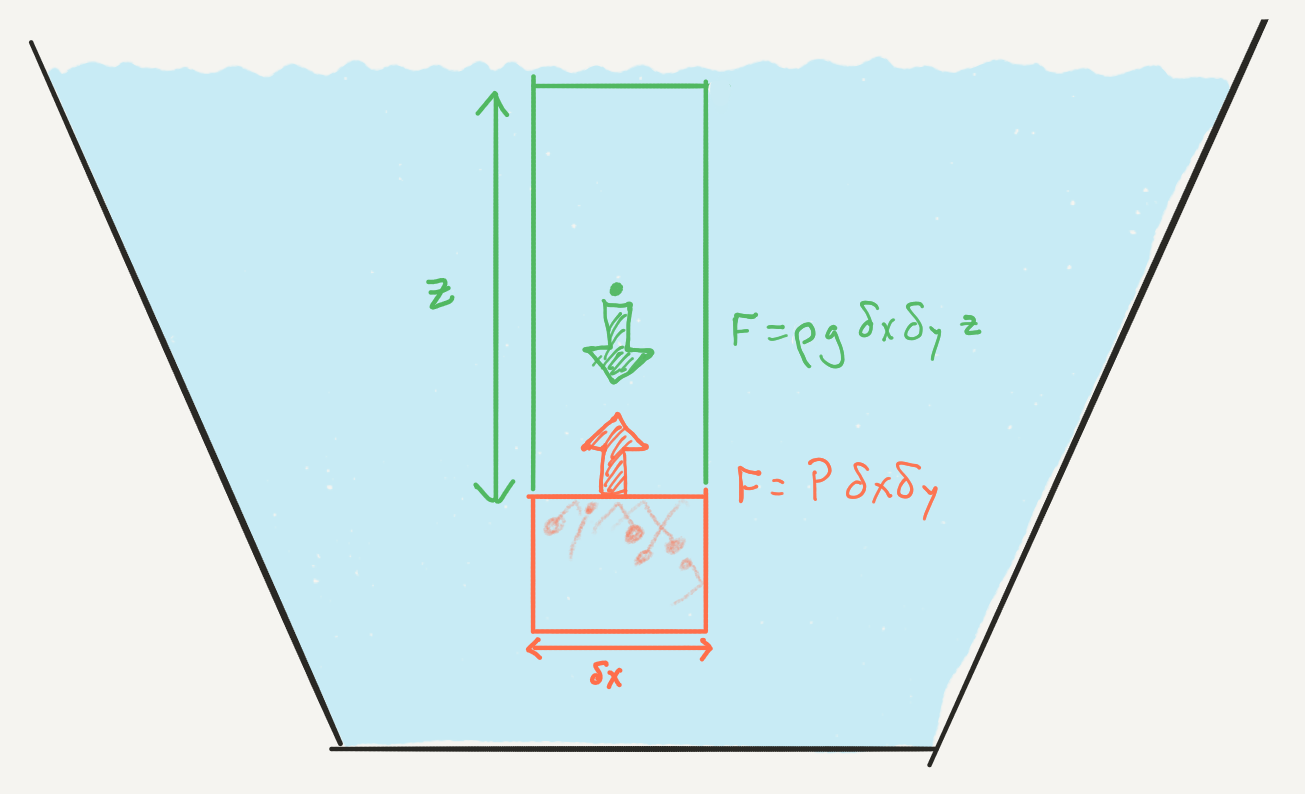
\includegraphics[width=3.5in]{figs/OneDens.png}
\caption{The pressure in the small orange box is  the weight per area of the water above.  $\delta y $ is in into the page, so $\delta x\ \delta y$ is the area of the top of the fluid parcel.  If the green column of water is static, then the two forces are equal and opposite.  }
\label{fig:OneDens}
\end{figure}


\subsection{Single density fluid}
``Hydrostatic pressure'' is the pressure water parcels exert on one another when the water is not moving.  Consider a
bucket of water, and think about the forces on a little ``cube''  of
water inside the bucket (\fref{fig:OneDens}, orange cube).  Suppose our cube is 0.1 m deep in the
bucket. There is a column of water above our little cube that is not
moving.  The force of gravity wants to pull this column of water
down (\fref{fig:OneDens}, green arrow).  The force is simply $F_{w}=mg$, where $g=9.8\, \mathrm{m\,s^{-2}}$, the mass $m=\rho V$, where
$\rho = 1000\ \mathrm{kg\,m^{-3}}$ is the density of water, and $V$ is the
volume of the column of water $V = (0.1 \ \mathrm{m})\,\delta x\,\delta y$.  So, the water column
is pushing down with force 
\begin{eqnarray*}
F&=&\delta x\,\delta y\,(0.1\,\mathrm{m})\,
(9.8\ \mathrm{m\,s^{-2}})\,(1000\ \mathrm{kg\,m^{-3}})\\
&\approx &\delta x\,\delta y\ 980\ \mathrm{N\,m^{-2}}\\
F/A &\approx & 0.098\ \mathrm{dbar},
\end{eqnarray*}
where we have called $\delta x\, \delta y$ our area element (i.e. $\delta A$ from \fref{fig:Ballon}).   
What provides the force that holds this water up, against gravity?  Its the water in our small cube. This water provides a force from directly below $F_{p}=P\,\delta x\,\delta y$ (\fref{fig:OneDens}, orange arrow).  If the water is not moving, $F_{p}=-F_{w}$, so that the sum of forces in the vertical is zero.
We can use this deduction to calculate the pressure at a depth $h$:
\begin{equation}
P(z=-h) = \rho\,g\,h.
\end{equation}
In other words, the pressure is the weight of the water above, per unit area.

It is important to remember that the squishing from the top also causes squishing to the sides, so the water pressurized by the water above also exerts forces on the water in the horizontal direction.  If the water beside our small cube has the same pressure forces acting on it, then the water won't move.  

\subsection{Two-density fluid}

\begin{figure}[htbp]
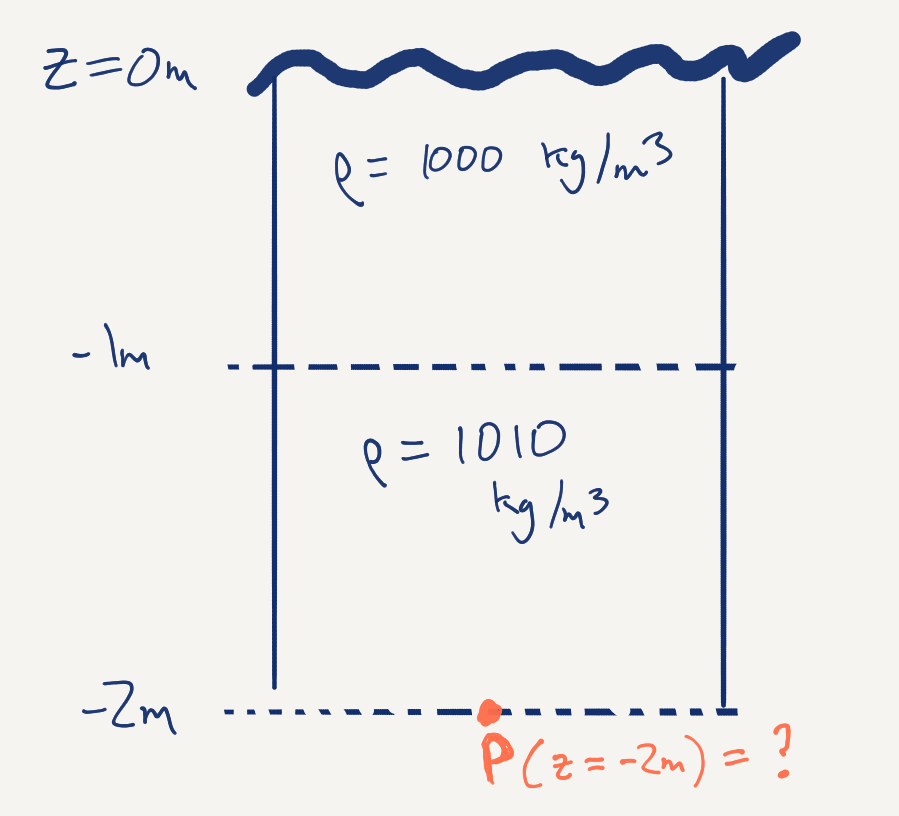
\includegraphics[width=2.7in]{figs/TwoDens.png}
\caption{Pressure in a two-layer fluid.  Imagine the first layer has a different density than the second, and that the densities are (approximately) constant in each layer.}
\label{fig:TwoDens}
\end{figure}

If the density of the water varies due to changes in temperature or salinity, then the weight needs to be calculated by summing up the different densities with depth.  i.e. imagine that the first meter, the density is $1000\ \mathrm{kg\,m^{-3}}$, and for the second meter, the density is $1010\ \mathrm{kg\,m^{-3}}$ (\fref{fig:TwoDens}).  Then the pressure at 2 m is:
\begin{eqnarray}
  P(z)&=&\int \rho(z)\,g\ \mathrm{d}z\\
  &\approx&\sum_{j=1}^{n} \rho_{j}\, g\ \Delta z_{j}\\
  & =& (1000\times1\times9.8\ +\ 1010\times1\times9.8) \ \ \mathrm{N\,m^{-2}}\\
  &=& 19698\ \mathrm{N\,m^{-2}}
\end{eqnarray}
Adding more layers to the water column, or making the layers different thicknesses is just handled by adding more terms to the sum.  Often it is useful to use a computer for this kind of calculation!

\section{Pressure gradients}
\subsection{Surface pressure gradients}
\label{sec:pressure-gradients}

We wouldn't care too much about pressure if it did not cause water to move.  Consider a sloshing bathtub, mid-slosh (\fref{fig:Bathtub}).  In this situation it is intuitively obvious that the water wants to move from left to right, but what force is pushing it?  First, where is pressure the highest at point A or point B?   These points are both a depth $h$ below the \emph{resting} depth of the surface of the fluid.  Above point A, there is slightly more water due to the ``slosh'', whereas above point B there is slightly less.  Therefore the pressure at point A is greater than at point B.  ($P_{A}(z=-h) = \rho g (h+\eta_{A})$ and $P_{B}(z=-h) = \rho g (h+\eta_{B})$, where $\eta$ is the height of the water above its resting depth. $\eta_{A}>0$, and $\eta_{B} <0$, therefore $P_{A}>P_{B}$).

It should also be obvious that \emph{everywhere} in the fluid the pressure is decreasing to the right along any given depth i.e. $dP/dx<0$.  In fact the \emph{horizontal pressure gradient} can be calculated from
\begin{equation}
P(z=-h) = \rho g (h+\eta)
\end{equation}
and taking the derivative to get the gradient:
\begin{equation}
\frac{\mathrm{d}P}{\mathrm{d}x}(z=-h) = \rho g \frac{\mathrm{d}\eta}{\mathrm{d}x}.
\end{equation}
or, the change in the pressure is caused by the slope of the sea surface, $\mathrm{d}\eta / \mathrm{d}x$.

\begin{figure}[htbp]
\begin{center}
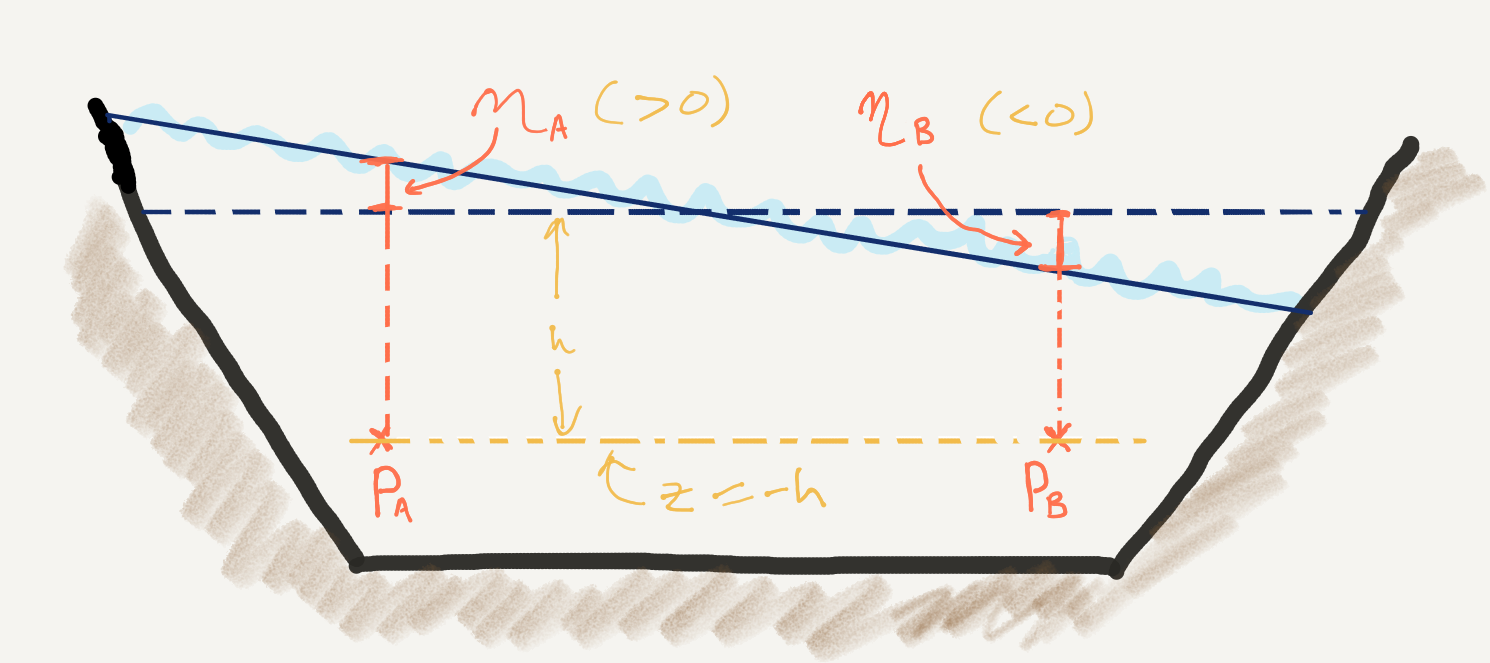
\includegraphics[width=4in]{figs/Bathtub.png}
\caption{Pressure in a sloshing tub.  For pressure gradients, we always compare the pressure at the same distance from the surface of the \emph{if it was flat} (i.e. the geoid), which here we have denoted $z=-h$.  The sea surface is described as the anomaly from this flat surface, $\eta >0 $ means the surface is above the flat level, and $\eta<0$ means that it is below.}
\label{fig:Bathtub}
\end{center}
\end{figure}

How does this move the water?  Lets consider the force diagram on a block of water inside the tub (\fref{fig:ForceDia})  If the pressure is greater on the left hand side, then the force into the block from the left is larger than the force into the block on the right, and the net force $F_{A}-F_{B}>0$, and the block tends to move to the right.  Note that in this case $\mathrm{d}P/\mathrm{d}x<0$.  

Recall Newton's second law of motion:
\begin{equation}
    \sum_{i=1}^{N} F_i = m \frac{du}{dt}
\end{equation}
where $du/dt$ is the acceleration (change of velocity with time).  For our block, $m = \rho\ \delta x\ \delta y\ \delta z$,  and $F_A = P_A \ \delta y\ \delta z$, and $F_B = - P_B \ \delta y\ \delta z$, so:
\begin{equation}
    P_A - P_B = \rho\ \delta x\ \frac{du}{dt}
\end{equation}
or, as $\delta x$ is made very small:
\begin{equation}
\frac{\mathrm{d}u}{\mathrm{d}t} = -\frac{1}{\rho}\frac{\mathrm{d}P}{\mathrm{d}x} + (\mathrm{other\ Forces\ in\ x})
\end{equation}
A question for the reader is to check that this gives the correct sign of the acceleration compared to their intuition.

\begin{figure}[htbp]
    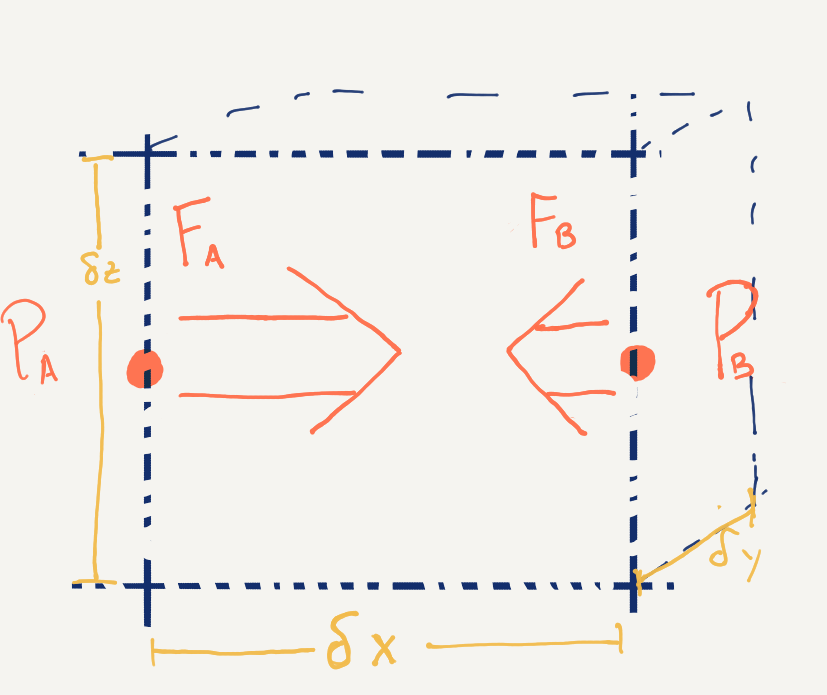
\includegraphics[width=3in]{figs/ForceDia.png}
    \caption{Lateral forces across a small hypothetical block.}
    \label{fig:ForceDia}
\end{figure}


For the example of the bathtub given above, it should also hopefully be clear that the pressure gradient, and thus the acceleration, does not depend on the depth below the surface.  The pressure gradient, $dP/dx$, only depends on the sea surface tilt, not on $z$.

\subsection{Internal pressure gradients}

If the fluid has varying density, then the pressure field can be more complicated, and the motions harder to predict.  For the simplest case, consider a two-layer fluid, with a flat upper surface, and a tilted interface between two layers with densities $\rho_{1}$ and $\rho_{2}$ (\fref{fig:TwoLayer}) with $\rho_{2}>\rho_{1}$.  Again, the pressure is lower on the right than left, so water in the deeper layer has a pressure gradient force from high pressure to low pressure, i.e. to the right.
\begin{figure}[htbp]
\begin{center}
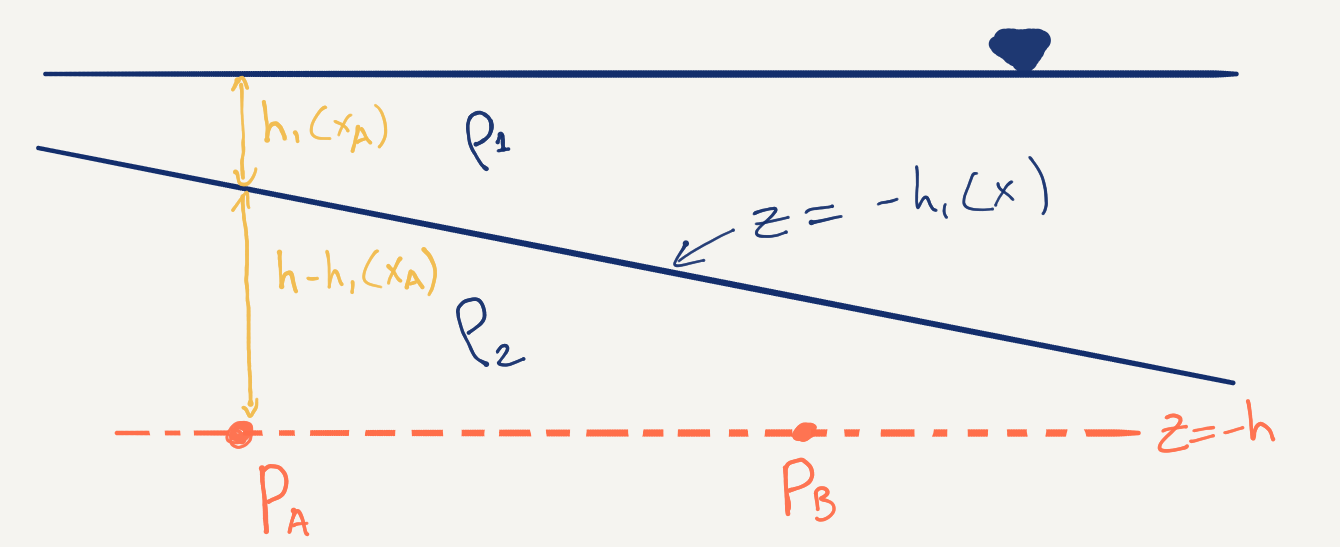
\includegraphics[width=4in]{figs/TwoLayer.png}
\caption{How to calculate the pressure gradient in a two-layer fluid.}
\label{fig:TwoLayer}
\end{center}
\end{figure}

Mathematically, $P_{A}(z=-h) = g(\rho_{1} h_{1}(x_{A}) + \rho_{2} (h-h_{1}(x_{A})))$, and
$P_{B}(z=-h) = g(\rho_{1} h_{1}(x_{B}) + \rho_{2} (h-h_{1}(x_{B})))$.  We can estimate the pressure gradient as
\begin{equation}
\frac{\mathrm{d}P}{\mathrm{d}x} \approx \frac{P_{B}-P_{A}}{x_{B}-x_{A}} = g(\rho_{1}-\rho_{2})\frac{h_{1}(x_{B})-h_{1}(x_{A})}{x_{B}-x_{A}} = -g(\rho_{2}-\rho_{1})\frac{\mathrm{d}h_1}{\mathrm{d}x}
\end{equation}
So again, the pressure gradient depends on the slope of the interface, except this time, the interface is between the two densities.

Of course, the cases can be combined (\fref{fig:MultipleLayers}).  There can be a surface tilt, and many interface tilts.  While care needs to be taken to keep track of all the layer thicknesses, and the algebra looks messy on the page, the fundamental idea is to simply calculate the weight of the water about the point of interest, including the effect of the local sea-surface elevation.

\begin{figure}[htbp]
\begin{center}
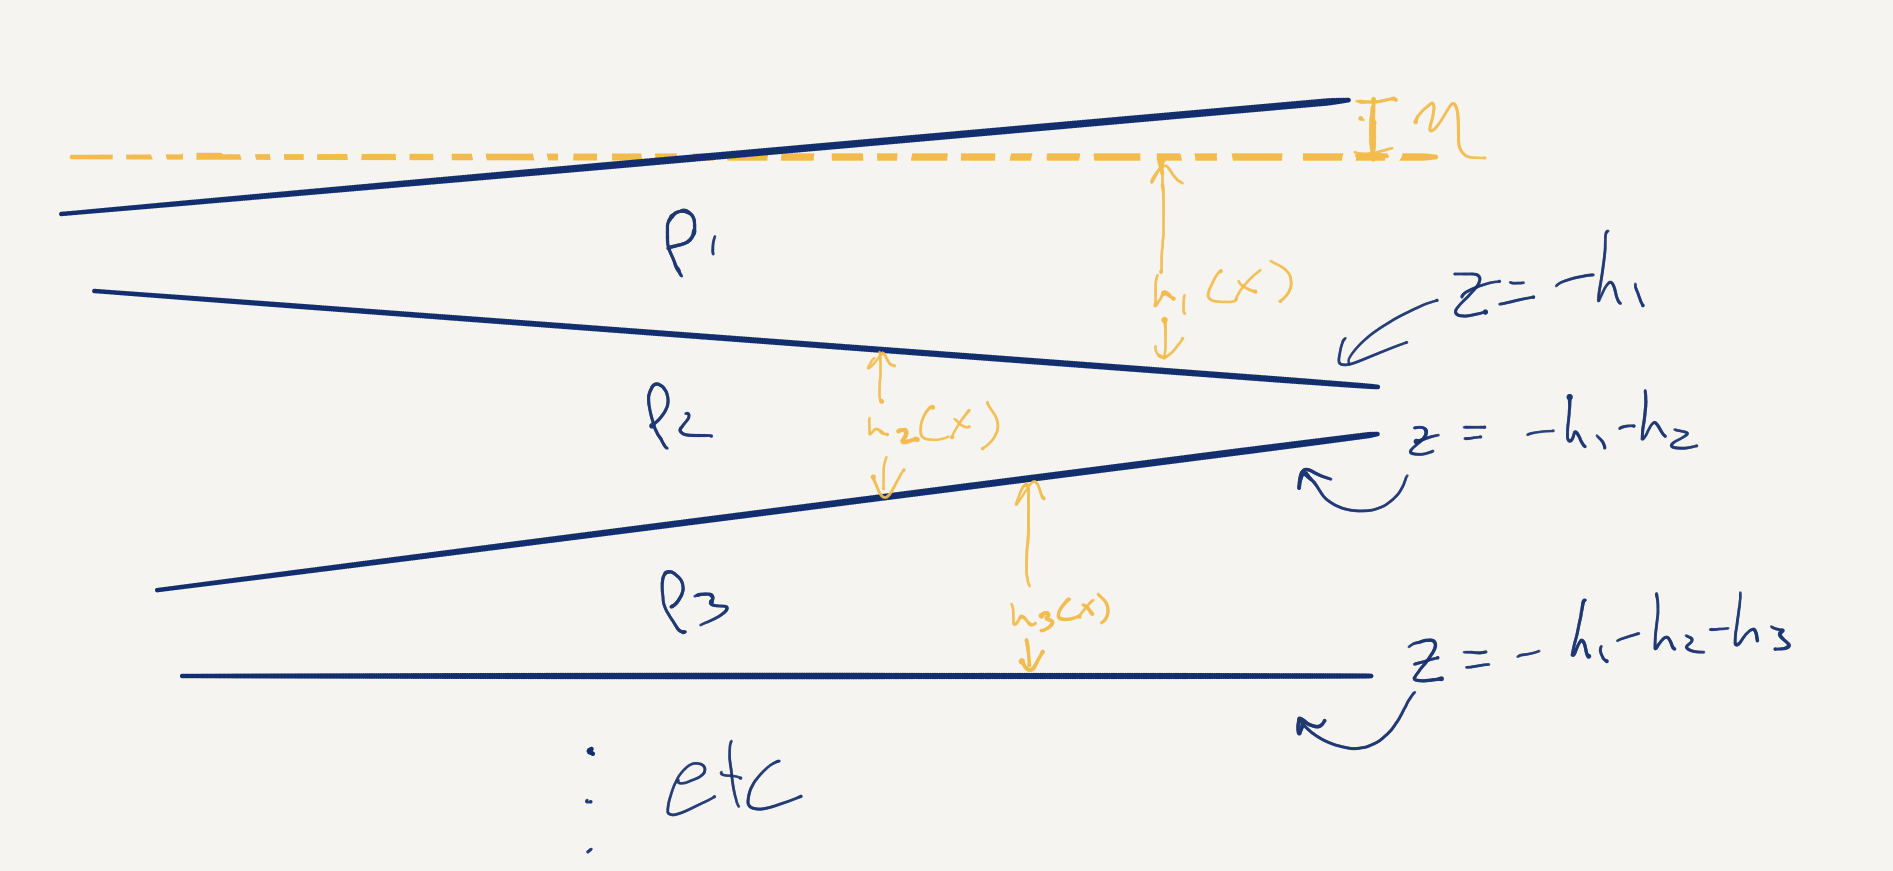
\includegraphics[width=4in]{figs/MultipleLayers.png}
\caption{Many-layer fluid.}
\label{fig:MultipleLayers}
\end{center}
\end{figure}

\clearpage
\section{Exercise}

A cruise goes out and makes temperature measurements at two locations 25 km apart as follows:

  \begin{tabular}{l|cc}
    $z$& $T_A$& $T_B$\\
    \hline
    10 & 10.4& 10.1 \\
    30 & 8.7 & 8.4\\
    50 & 4.7 & 5.2\\
    70 & 4.1 & 4.8\\
  \end{tabular}
The density of fresh water at $10\mathrm{^oC}$ is $1008\ \mathrm{kg\,m^{-3}}$.  What is the \emph{approximate} density at each location where a temperature measurement was taken?

What direction would you expect the water to be flowing at each depth?

Approximate the strength and sign of the horizontal hydrostatic pressure \emph{gradient} at 20, 40, 60 and 80 m, assuming a flat sea surface. Make sure you write out the equation so I can check your math. Does your answer make sense with the answer above? Hint: discretize the water column by assuming that it consists of 4 20-m layers of water, each with a constant temperature. Also, don't round off your density values too much!

What must the difference in the sea surface height be at the two stations for your estimated horizontal pressure gradient to be zero at 40 m?

%%% Local Variables:
%%% mode: latex
%%% TeX-master: t
%%% End:
